\documentclass{article}
\usepackage[utf8]{inputenc}
\usepackage[spanish]{babel}
\usepackage{graphicx, graphics, float, hyperref}
\usepackage{listings}
\usepackage[a4paper, total={6in, 10in}]{geometry}

\title{DSD Memoria Práctica 4}
\author{Andrés Merlo Trujillo}
\date{}
\hypersetup{
    colorlinks=true,
    linkcolor=black,
}

\begin{document}
%TODO: COMPROBAR EN LA PARTE DE SOCKET IO QUE PARTES SON EXACTAMENTE SOCKETS.
%TODO 2: MEJORAR LA EXPLICACIONES EN GENERAL, SOBRE TODO LA PARTE DE LOS SOCKETS QUE ESTA MUY RARA.

\maketitle

\tableofcontents

\newpage

\section{Introducción}
En esta práctica se pide probar unos ejemplos de prueba y comentarlos, e implementar un sistema de domótica básico.

Para ello, es necesario tener instalado Node.js y MongoDB. También es necesario instalar npm para poder instalar los módulos de Socket.io y el de MongoDB (driver para la conexion con la BB.DD.).

Un problema que he tenido ha sido que no podía ejecutar el archivo de prueba \textit{mongo-test.js}. Mostraba el mensaje de que el servidor se había iniciado, pero al intentar acceder con la URL ponía que la conexión había sido rechazada. Tras pasar un periodo de tiempo de unos 40 segundos, el programa mostraba un mensaje de error.

Tras depurar el programa en busca del mensaje de error, me di cuenta que localhost se resolvía a \textit{::1}, que es la versión IPv6. Además al hacer ping a localhost obtenía lo siguiente:

\begin{figure}[H]
    \centering
    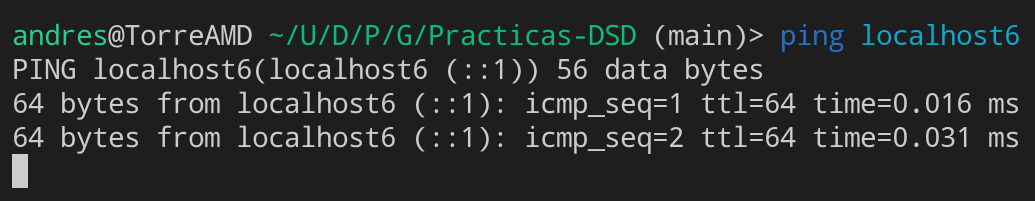
\includegraphics[width=0.7\textwidth]{images/ping.png}
    \caption{Salida que salía. Al estar arreglado sale localhost6, pero ponía localhost antes.}
\end{figure}

Por tanto siempre se estaba resolviendo a la dirección IPv6.

MongoDB por defecto no usa IPv6, por lo que hay dos opciones para que funcione:

\begin{itemize}
    \item Permitir a MongoDB que use también las direcciones IPv6 o.
    
    \item Modificar el archivo \textit{/etc/hosts} para que use otro nombre distinto.
\end{itemize}

AL final opté por la segunda opción. Para ello llamé a ``localhost'' en IPv6 como ``localhost6''. Ahora al hacer ping sí se obtiene la dirección loopback de IPv4:

\begin{figure}[H]
    \centering
    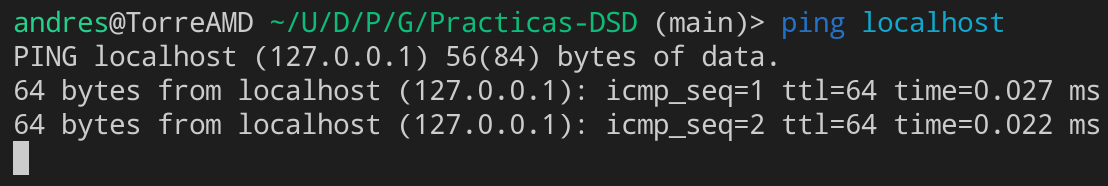
\includegraphics[width=0.7\textwidth]{images/pingOk.png}
    \caption{Salida después del arreglo.}
\end{figure}

%QUIZAS SI DA MAS FALLOS MONGO PONERLOS

\section{Primera parte. Ejemplos}
\subsection{helloworld.js}
\subsubsection{Descripción}
Este ejemplo lo único que realiza es mostrar por pantalla en el navegador el mensaje ``Hola mundo''.

Adicionalmente, también muestra por la terminal del servidor el JSON con toda la información de la petición del cliente (navegador).

\begin{figure}[H]
    \centering
    \begin{minipage}[H]{0.49\textwidth}
        \centering
        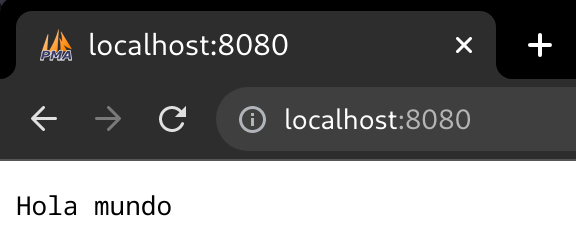
\includegraphics[width=\textwidth]{images/helloworldC.png}
        \caption{Salida del cliente.}
    \end{minipage}
    \hfill
    \begin{minipage}[H]{0.49\textwidth}
        \centering
        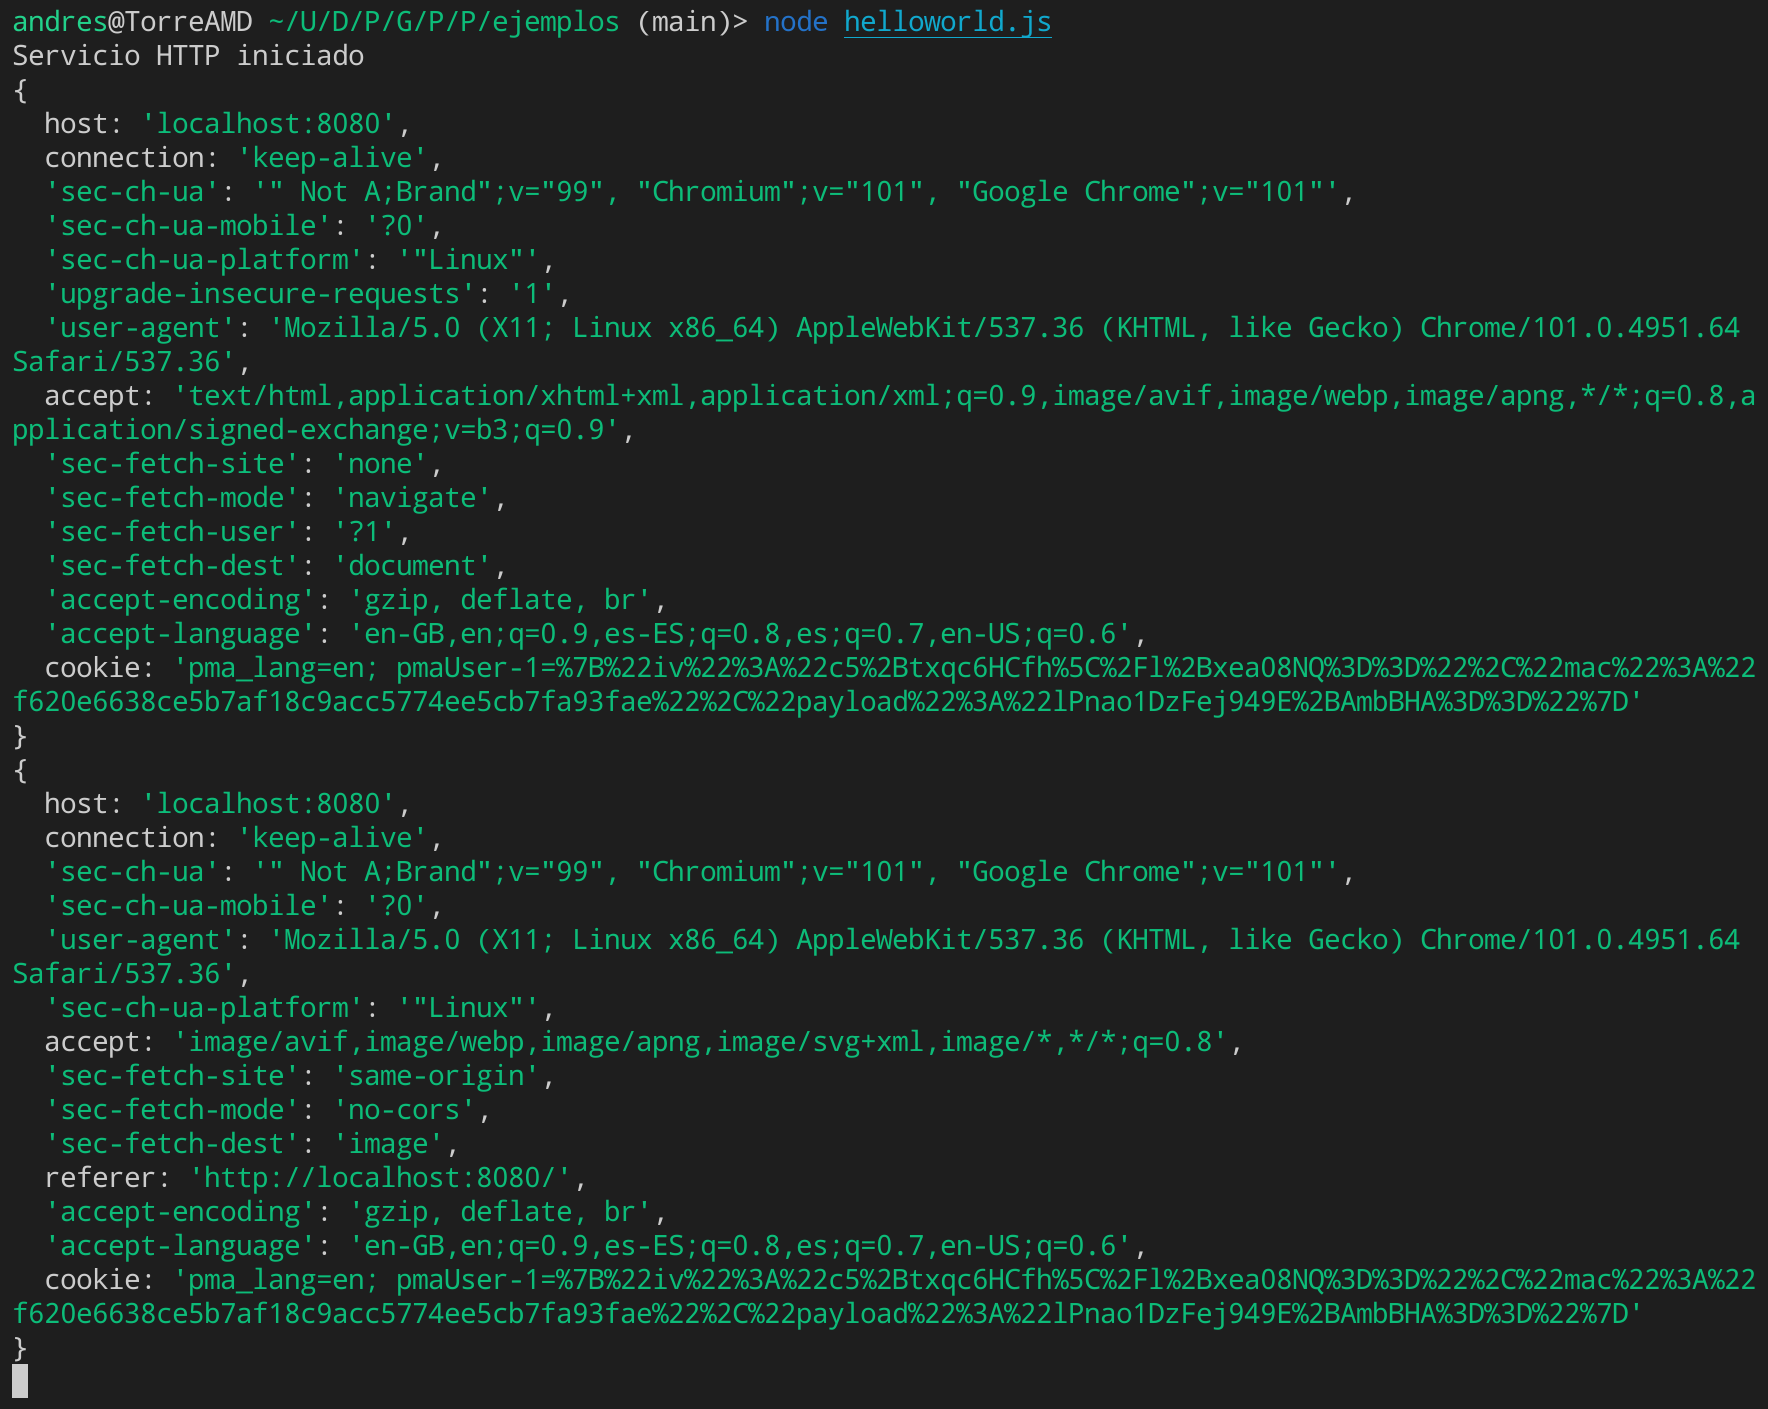
\includegraphics[width=\textwidth]{images/helloworldS.png}
        \caption{Salida del servidor.}
    \end{minipage}
\end{figure}

\subsubsection{Implementación}
Para realizar esto, lo primero que hay que hacer es montar el servidor HTTP. Para ello, se importa el módulo de Node.js ``http''.

Una vez importado, se crea el servidor con el método ``createServer'' cuyo argumento es una función que se ejecuta cada vez que se realiza una petición HTTP.

Dentro del cuerpo de esta función, para que el servidor muestre la información de la petición, es necesario usar ``request.headers'' y pasarlo al log de la consola de JavaScript.

Para que el cliente reciba el mensaje, es necesario escribir una cabecera básica con el código 200, indicando que es correcto y el tipo MIME, que en este caso será texto plano.

Luego con el método write, se escribe el mensaje ``Hola mundo'' en el cliente. POr último, se finaliza con end para que se mande el mesanje. %IMPORTANTE COMPROBAR ESTO, SEGURAMENTE ESTE MAL

\begin{figure}[H]
    \centering
    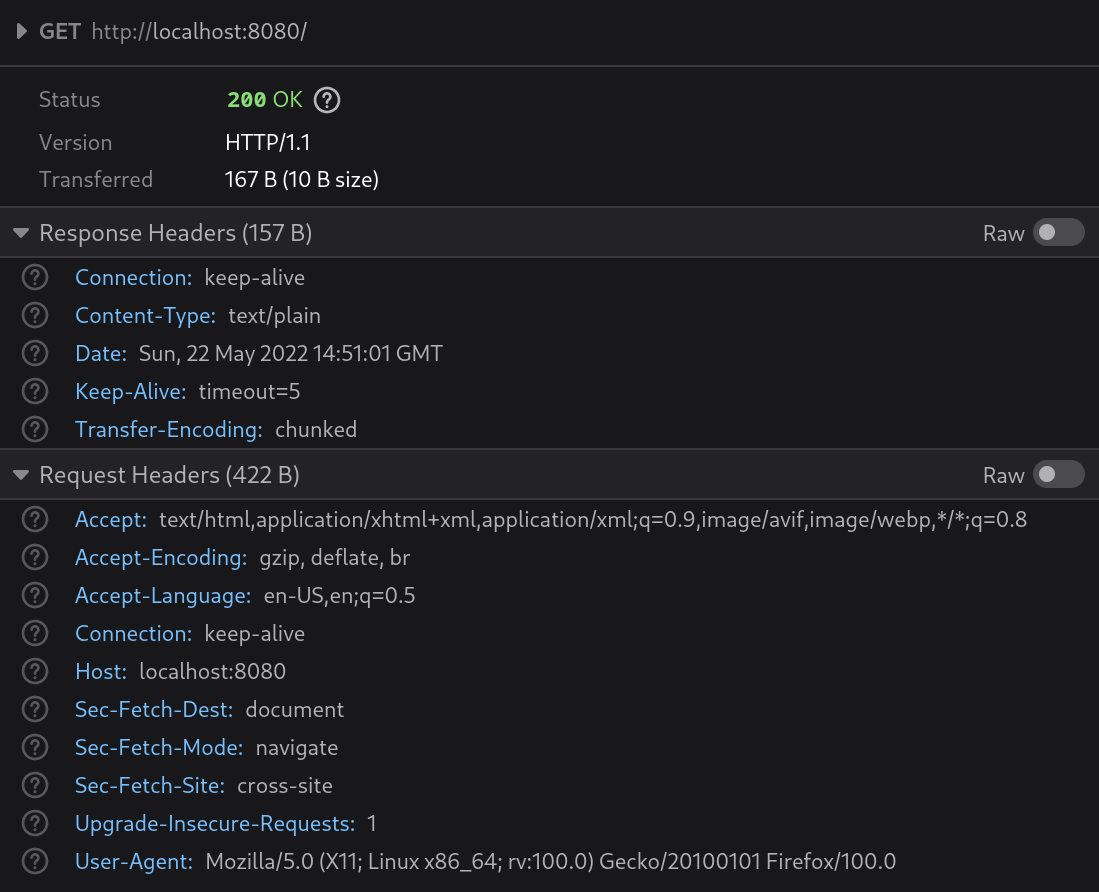
\includegraphics[width=0.7\textwidth]{images/header.png}
    \caption{Cabecera de la petición realizada en Firefox.}
\end{figure}

\subsection{calculadora.js}
\subsubsection{Descripción}
Este ejemplo implementa una calculadora básica haciendo uso de Node.js. 

A la calculadora se le pasa el operador y los operandos en la URL en el navegador. En caso de ser incorrectos o no tener suficientes, muestra en el navegador un error.

Las operaciones que puede hacer son: sumar, restar, producto y dividir.

La sintaxis de la URL es la siguiente: 

\verb|http://localhost:8080/<operador>/<operando-1>/<operando-2>|


\begin{figure}[H]
    \centering
    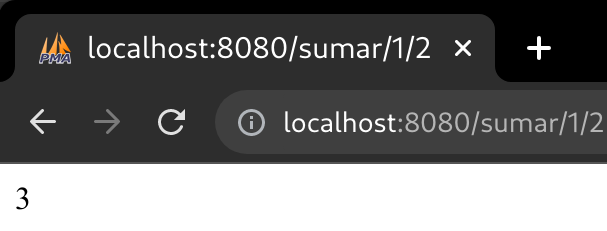
\includegraphics[width=0.4\textwidth]{images/rescalcnormal.png}
    \caption{Resultado de sumar 1 y 2 en Chrome.}
\end{figure}

\subsubsection{Implementación}
La parte de creación del servidor es exactamente igual que en la que se realiza en ``helloworld.js''.

Se ha creado una función ``calcular'' que permite realizar las funciones de la calculadora.

Tambień se usa el módulo ``url'' para obtener la URL que pasa el cliente. El objetivo es conseguir obtener los parámetros para pasarlos a la función y que realice la cuenta. Para ello, se usa ``url.parse'' con el ``request.url'' para obtener mas informacion de la URL y luego solo se escoge el campo ``pathname''. Esto hace que se obtenga la URI, por ejemplo, si se quiere hacer ``1+2'': ``/sumar/1/2''.

Cabe notar que, en este caso, la línea que hace esto es innecesaria, ya que se puede hacer un simple ``request.url'' y obtener la URI deseada.


Luego, se elimina el primer ``/'' para poder hacer luego split con el mismo delimitador para obtener un array con el operador el primero, y los operadores al final.

A continuación, se pasa a float y se llama a la funcion ``calcular''.

Por último, se manda de manera idéntica a la explicada en la sección anterior para el ``helloworld.js''.

\begin{figure}[H]
    \centering
    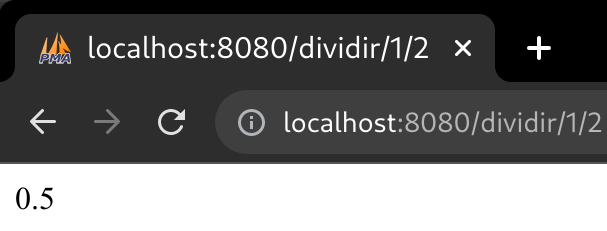
\includegraphics[width=0.4\textwidth]{images/dividircnormal.png}
    \caption{Resultado de dividir 1 entre 2 en Chrome.}
\end{figure}


\subsection{calculadora-web.js}
\subsubsection{Descripción}
Este ejemplo implementa exactamente lo mismo que ``calculadora.js'', pero teniendo una interfaz web que simplifica la introducción de los valores.

Tmbien hace uso de Node.js y de los módulos adicionales ``path'' y ``fs'' para buscar el archivo HTML con la ruta absoluta y también para comprobar la existencia de archivos en el sistema y de leerlos para ofrecerlos en el cliente.

\begin{figure}[H]
    \centering
    \begin{minipage}[H]{0.49\textwidth}
        \centering
        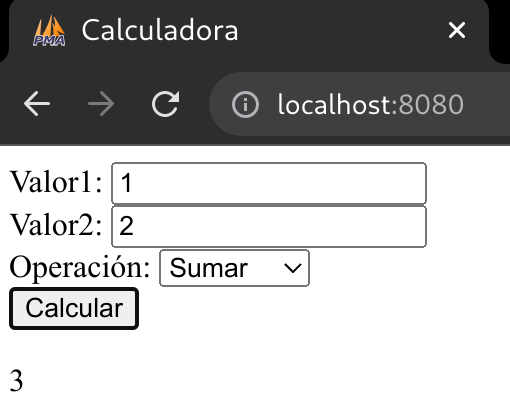
\includegraphics[width=\textwidth]{images/cwebsuma.png}
        \caption{Resultado de sumar 1 y 2 en Chrome.}
    \end{minipage}
    \hfill
    \begin{minipage}[H]{0.49\textwidth}
        \centering
        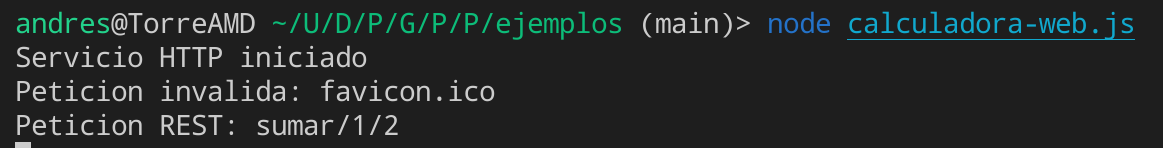
\includegraphics[width=\textwidth]{images/cwebsumaserver.png}
        \caption{Salida del servidor.}
    \end{minipage}
\end{figure}


Además muestra por la pantalla donde se ejecuta la petición REST que se ha realizado, que sigue la misma sintaxis que el ejemplo anterior.

\subsubsection{Implementación}
La implementacion es muy similar al anterior, pero en este caso se usa el modulo de Node.js ``fs'' para poder realizar operaciones con archivos.

Lo primero que tiene que hacer es enviar la pagina al navegador. Para ello, se consigue la URI como antes, luego se comprueba que si el usuario solo ha puesto la direccion (en este caso localhost:8080), en caso afirmativo se pone que sirva el archivo HTML. A continuación, se le añade la ruta absoluta de ese archivo y, finalmente, con el método ``exists'' comprueba que existe, y en caso afirmativo, con el método ``readFile'' se carga el archivo HTML de una manera similar a como se hacía para los mensajes en los ejemplos anteriores.

Una vez cargada la página, el usuario puede insertar los operandos y el operador y, al darle a enviar se ejecuta la función ``enviar'' que lo que hace es convertir los valores introducidos en una cadena del tipo ``operador/operando1/operando2''. LUego, realiza una petición HTTP GET al servidor con esta cadena, la cual al pasar por el método ``exists'' va a devolver que no existe porque no es un archivo y va a ejecutar el mismo código que en el ejemplo de la calculadora anterior, devolviendo asi el resultado de la operacion.

\begin{figure}[H]
    \centering
    \begin{minipage}[H]{0.49\textwidth}
        \centering
        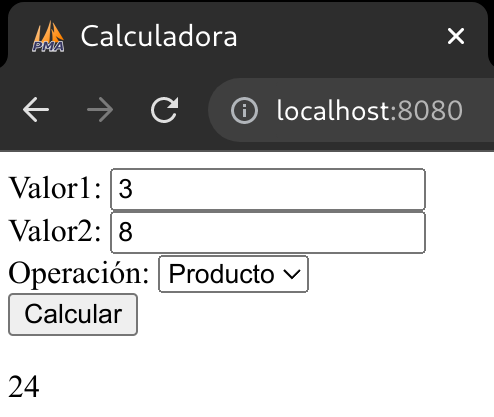
\includegraphics[width=\textwidth]{images/cwebprod.png}
        \caption{Resultado de multiplicar 3 por 8 en Chrome.}
    \end{minipage}
    \hfill
    \begin{minipage}[H]{0.49\textwidth}
        \centering
        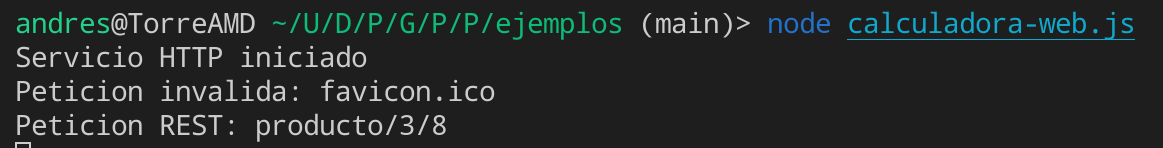
\includegraphics[width=\textwidth]{images/cwebprodserver.png}
        \caption{Salida del servidor.}
    \end{minipage}
\end{figure}

\subsection{connections.js}
\subsubsection{Descripción}
Este ejemplo hace uso del modulo Socket.io para poder actualizar todos los clientes de manera asíncrona y realizar una comunicación entre el cliente y el servidor para que todos tengan la información mas actualizada.

Cuando un cliente se conecta, este aparece en la pantalla del navegador con su direccion IP y el puerto usado. Además, si se abren mas pestañas se puede ver como aparece la direccion y puerto del nuevo cliente, junto a los que ya estaban conectados. Si nos dirigimos de nuevo a la pestaña del primer cliente se puede ver que se actualizan las conexiones también. Esto mismo pasa tambien para las desconexiones, cuando un cliente se desconecta los demás lo ven en su sesión.

En la pantalla del servidor aparecen los clientes conectados, las nuevsas conexiones y cuando un usuario se va a desconectar.

\begin{figure}[H]
    \centering
    \begin{minipage}[H]{0.49\textwidth}
        \centering
        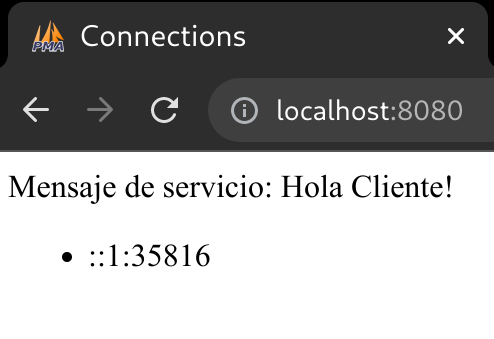
\includegraphics[width=\textwidth]{images/connect1.png}
        \caption{Un solo cliente conectado.}
    \end{minipage}
    \hfill
    \begin{minipage}[H]{0.49\textwidth}
        \centering
        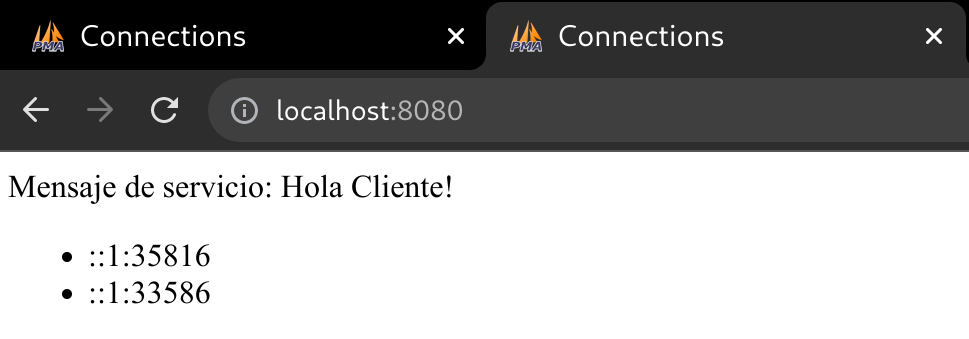
\includegraphics[width=\textwidth]{images/connect2.png}
        \caption{Dos clientes conectados}
    \end{minipage}
\end{figure}

Además, cuando se desconecta el servicio, aparece un mensaje informandolo.

\begin{figure}[H]
    \centering
    \begin{minipage}[H]{0.49\textwidth}
        \centering
        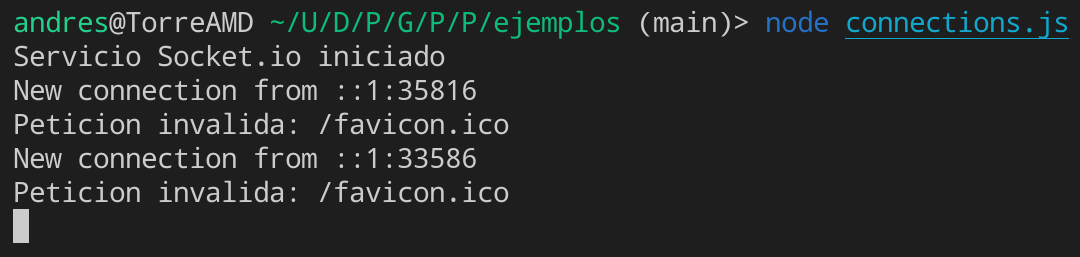
\includegraphics[width=\textwidth]{images/connectserver.png}
        \caption{Salida del servidor cuando se conectan dos.}
    \end{minipage}
    \hfill
    \begin{minipage}[H]{0.49\textwidth}
        \centering
        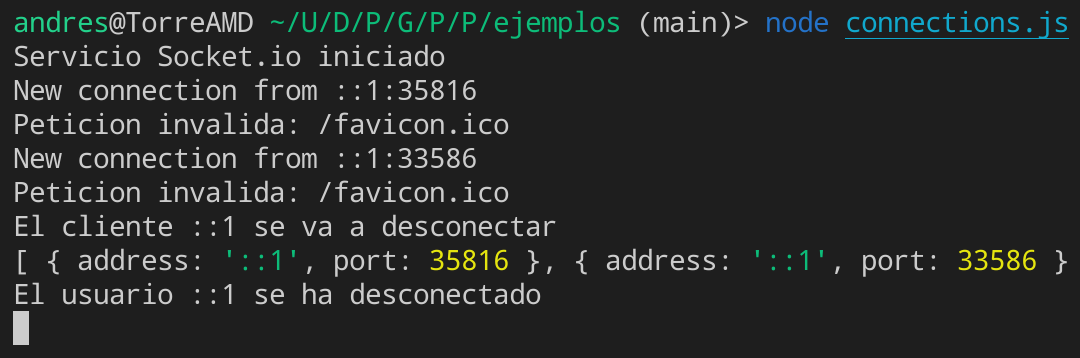
\includegraphics[width=\textwidth]{images/disconnectserver.png}
        \caption{Salida del servidor cuando un cliente se desconecta.}
    \end{minipage}
\end{figure}

\subsubsection{Implementación}
Para implementar este ejemplo es necesario crear un ``httpServer'' como se ha hecho en los ejemplos anteriores, pero esta vez sólo cargando el fichero html.

También es necesario crear el objeto Socket.io e indicarle la funcionalidad y los eventos que debe escuchar y emitir en cuanto se conecte un cliente. En este caso, cuando un cliente se conecta, lo que se hace primero es añadir el usuario al array, luego se emite a todos los suscritos el cambio y por último se configuran los eventos de escucha ``output-evt'' y ``disconnect'' para mostrar un mensaje por el navegador y para actualizar los clientes conectados respectivamente, cuando el cliente emita alguno de estos eventos.

En el fichero HTML se conencta al socket del servidor y se configuran los eventos que va a suscrbirise. El evento ``connect'' se ejecuta en cuanto se conecta y le manda un evnto del tipo ``output-evt'' al servidor, el cual devuelve de vuelta ``Hola Cliente!'' y lo capta el cliente en ``output-evt'', que actualiza el mensaje de la página HTML.

Cuando un cliente se desconecta se ejecuta en el servidor el evento ``disconnect'', el cual elimina al cliente de la lista y manda a todos los clientes el evento ``all-connections'' para que actualicen ellos también la lista.

Por último, todos los clientes tienen el evento ``disconnect'', que permite que cuando el servidor se caiga por diversos motivos, cambie el mensaje de la página.

%INTRODUCIR FOTOS DE SALIDA CON VARIOS CLIENTES Y TODO ESO, JUNTO CON LAS DEL SERVIDOR

%El diagrama de interacciones es el siguiente:

%MOSTRAR SI ME VEO CAPAZ EL DIAGRAMA DE INTERACCION.
\subsection{mongo-test.js}
\subsubsection{Descripción}
Este ejemplo muestra al cliente todas las conexiones a la base de datos NoSQL, mostrando en un JSON el identificador, la dirección IP donde se encuentra el cliente, el puerto y la hora UTC a la que se ha realizado la conexión.

Cuando se refresca la página o se abre una pestaña nueva del navegador, aparecen nuevas líneas de conexiones a la base de datos.

%Mostrar una foto de la salida
\begin{figure}[H]
    \centering
    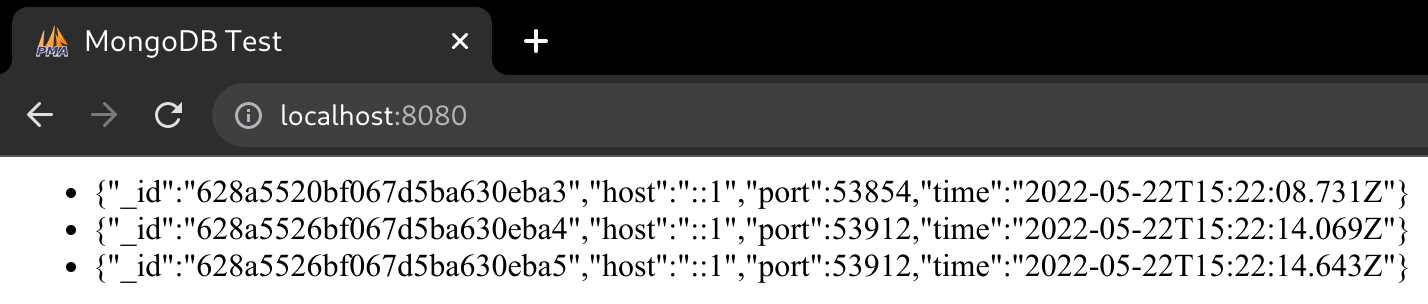
\includegraphics[width=0.7\textwidth]{images/mongo3.png}
    \caption{Tres conexiones distintas al servidor.}
\end{figure}

\subsubsection{Implementación}
La implementación del servidor HTTP es exactamente igual que en ejemplos anteriores, cuando se realiza una petición, el servidor envia la pagina HTML que se encarga de mostrar las conexiones.

En la parte de la base de datos, lo primero que se hace es conectarse, luego se crea una base de datos con nombre ``pruebaBaseDatos''.

A continuación, con Socket.io, se crean los eventos que tiene que escuchar y emitir: 

\begin{itemize}
    \item \textbf{my-address}: manda al cliente su dirección IP y puerto
    \item \textbf{poner:} Inserta los datos que el cliente manda en la base de datos.
    \item \textbf{obtener:} busca en la base de datos el registro dado por la dirección IP del cliente y se lo manda al mismo (el cliente).
    \item \textbf{poner:} Se encarga de insertar en la base de datos la informacion que ha enviado el cliente.
\end{itemize}

Para la parte del fichero HTML en el cliente, se realiza algo similar a ejemplos anteriores. Los eventos se encargan de insertar en la base de datos las nuevas conexiones y de actualizar la lista del cliente.

Ahora bien, debido a que se usa el método ``createCollection'', solo se puede ejecutar el servidor una vez, en las siguientes ejecuciones da el siguiente error:

\begin{figure}[H]
    \centering
    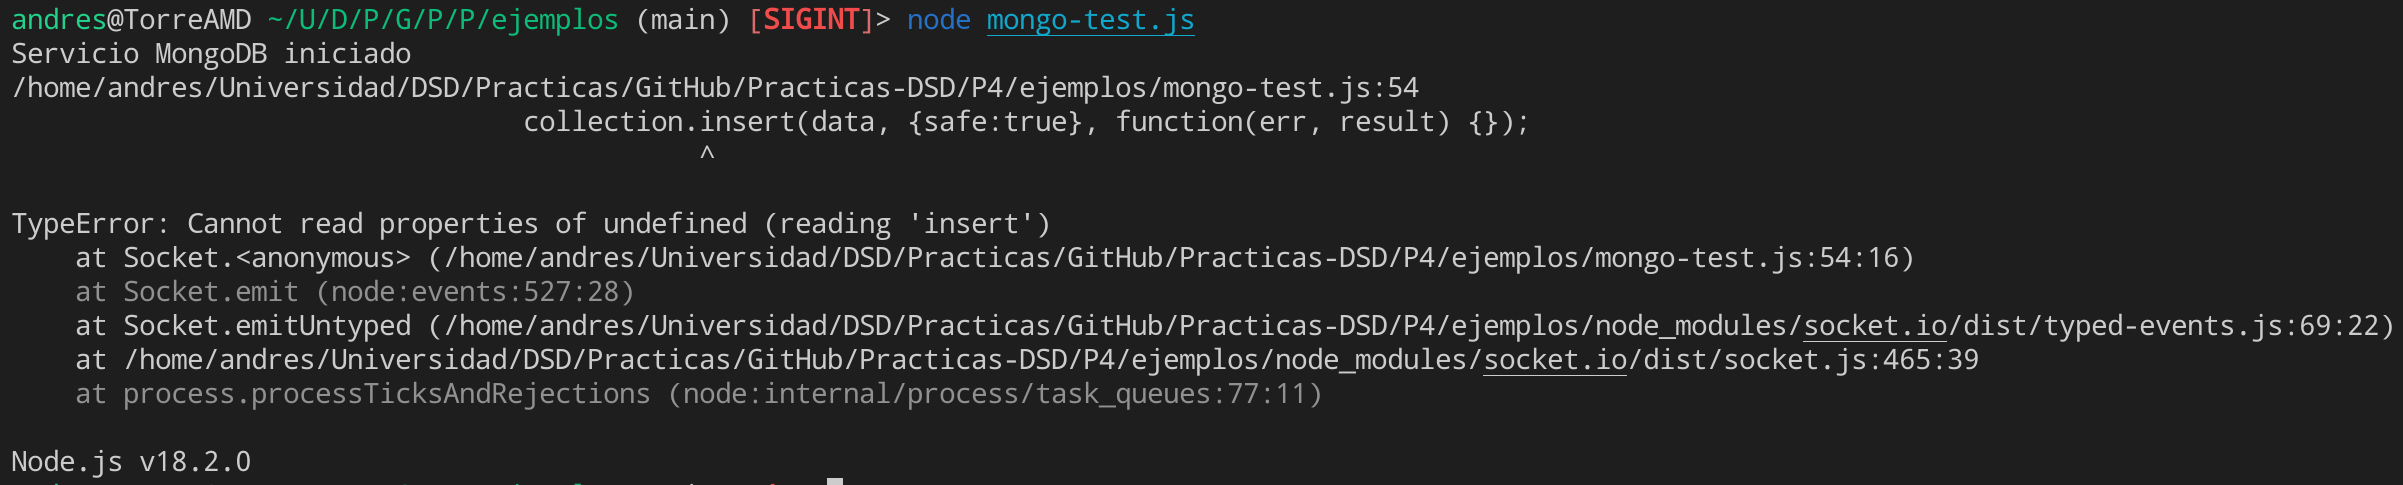
\includegraphics[width=0.8\textwidth]{images/errormongo.png}
    \caption{Error de ejecucion del servidor.}
\end{figure}

Esto es deido a que intenta crear de nuevo la coleccion y no lo consigue, haciendo que ``result'' sea ``null''.

\subsection{Diferencias entre los ejemplos}
La principal diferencia entre los distintos ejemplos, es que en algunos se hace uso de un fichero HTML dedicado con javascript incrustado para el cliente, mientras que en otros tales como ``helloworld.js'' o ``calculadora.js'', el servidor solo incrusta el mensaje en una página básica.

Otra diferencia es que ``helloworld.js'', ``calculadora.js'' y ``calculadora-web.js'' sólo hacen uso de Node.js, y algunos módulos del mismo. Mientras que en ``connections.js'' y ``mongo-test.js'' hacen uso de Socket.io adicionalmete.

Por último, ``mongo-test.js'' hace uso de un módulo (driver) para conectarse a una base de datos NoSQL. Por tanto, este es el mas complejo de todos.

\section{Segunda parte. Sistema domótico}
\subsection{Descripción}
En esta parte de la práctica se pide implementar un sistema de domotica basico que conste de dos sensores y dos actuadores. Los sensores reciben la informacion mediante un formulario, que en mi caso lo he hecho en una pagina aparte. Ademas deben mostrar alertas cuando los valores superen unos limites y en caso de llegar al limite de temperatura o luminosidad, se cierra la persiana automaticamente. Como extra, también he hecho que se accionen más actuadores en funcion de distintos valores de otros sensores.

Tambien he realizado algunos extras que explicare mas adelante para dotar al sistema de una mayor funcionalidad y autenticidad en la toma de decisiones sobre los actuadores.

\subsection{Implementación}
\subsubsection{Parte obligatoria}
Para esta parte lo que he hecho ha sido crear un servidor HTTP tal y como se realiza en los ejemplos proporcionados. Para la parte de la base de datos he realizado algo similar al ejemplo ``mongo-test.js'', he creado una base de datos denominada ``accionesSensores'' para almacenar todos los cambios que se realizan en los sensores a traves del formulario.

Debido a que el ejemplo anteriormente mencionado usaba el método ``createCollection'', cuando el servidor se reiniciaba y la coleccion ya existia se producia un error y se paraba la ejecucion del servidor. Tras revisar la documentacion al final encontre el metodo ``collection'', muy similar al anterior, pero con la diferencia de que no tiene funcion fallback (se almacena la referencia en una variable) y que al existir ya una coleccion, simplemente obtiene la referencia y no intenta crearla de nuevo. En caso de no existir, sí crea la coleccion y devuelve la referencia a la misma, asegurando así que nunca falle por intentarla crearla de nuevo.

Para la parte del agente, he realizado (solo en la parte basica, en la parte extra explicare la otra funcion) una funcion, denominada \textbf{PONER EL NOMBRE DE LA FUNCION AQUI}, que se encarga de comprobar que los valores sensores esten dentro de unos umbrales, y en caso de no estarlos, crea una nueva alerta y la manda al cliente.

La interfaz web he intentado que sea más o menos consistente en términos de colores y de diseño. Tiene la siguiente forma:

%MOSTRAR IMAGEN DE LA PANTALLA PRINCIPAL
\begin{figure}[H]
    \centering
    \begin{minipage}[H]{0.49\textwidth}
        \centering
        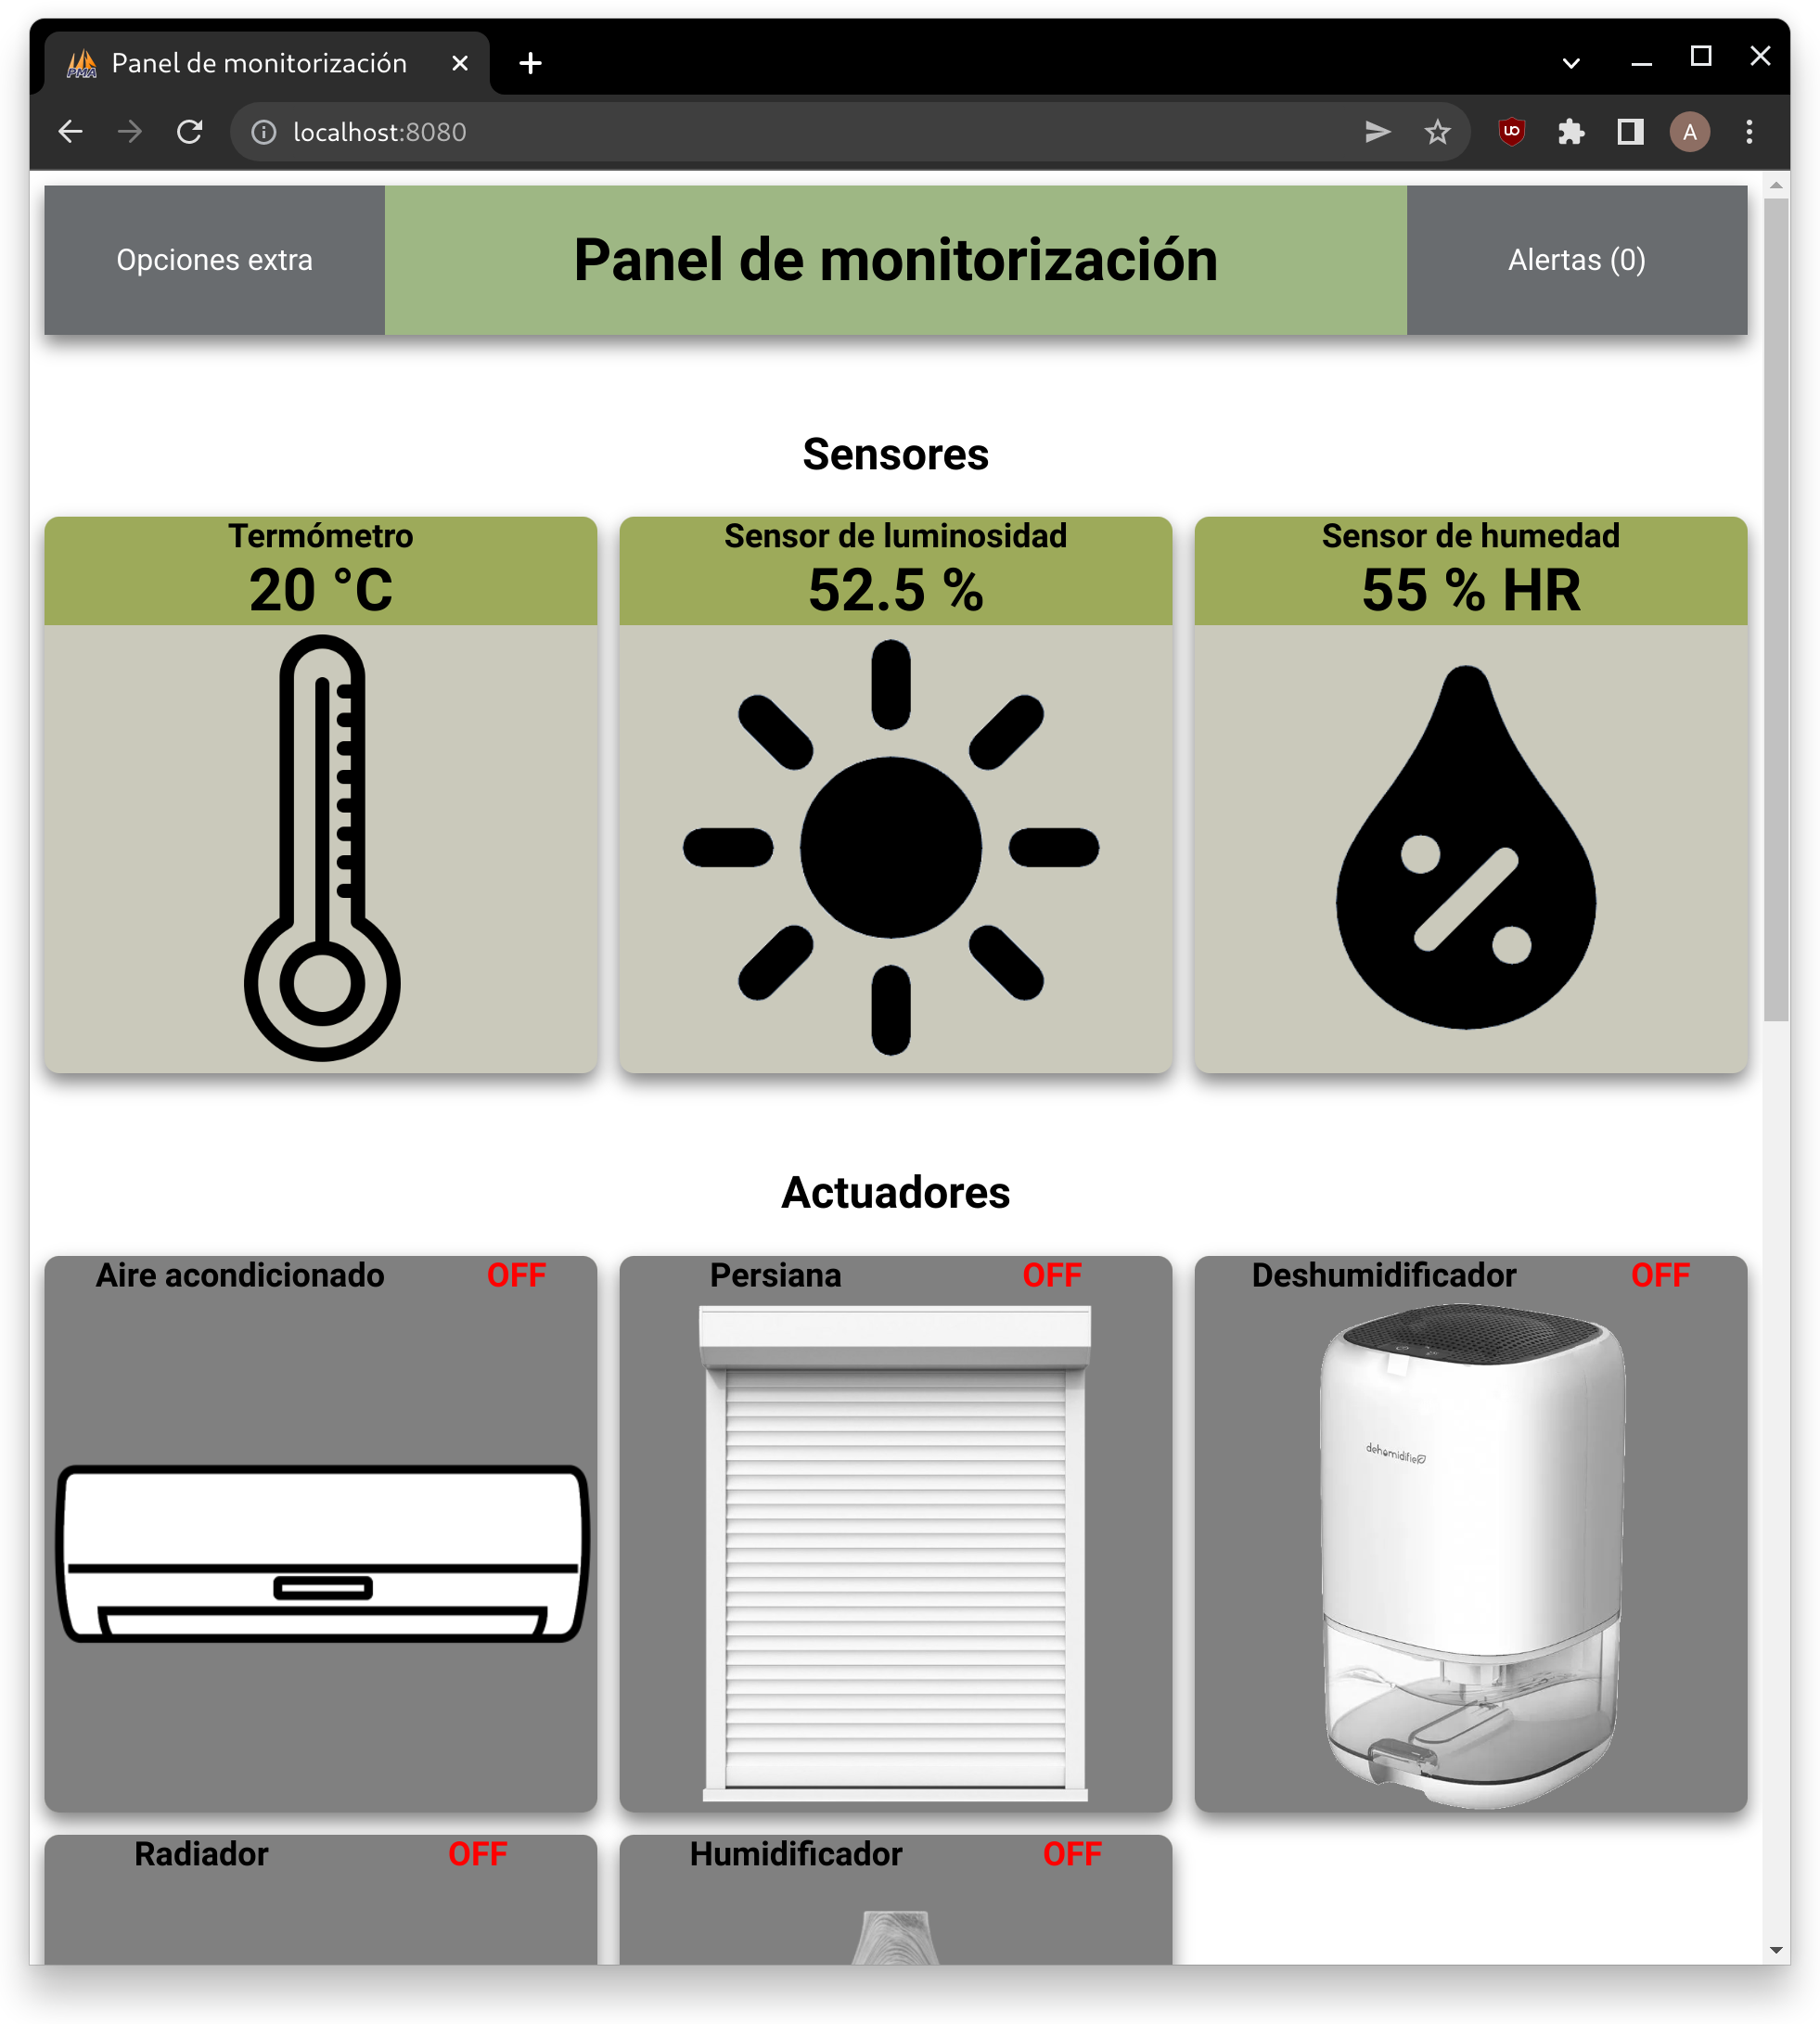
\includegraphics[width=\textwidth]{images/pagina1.png}
    \end{minipage}
    \hfill
    \begin{minipage}[H]{0.49\textwidth}
        \centering
        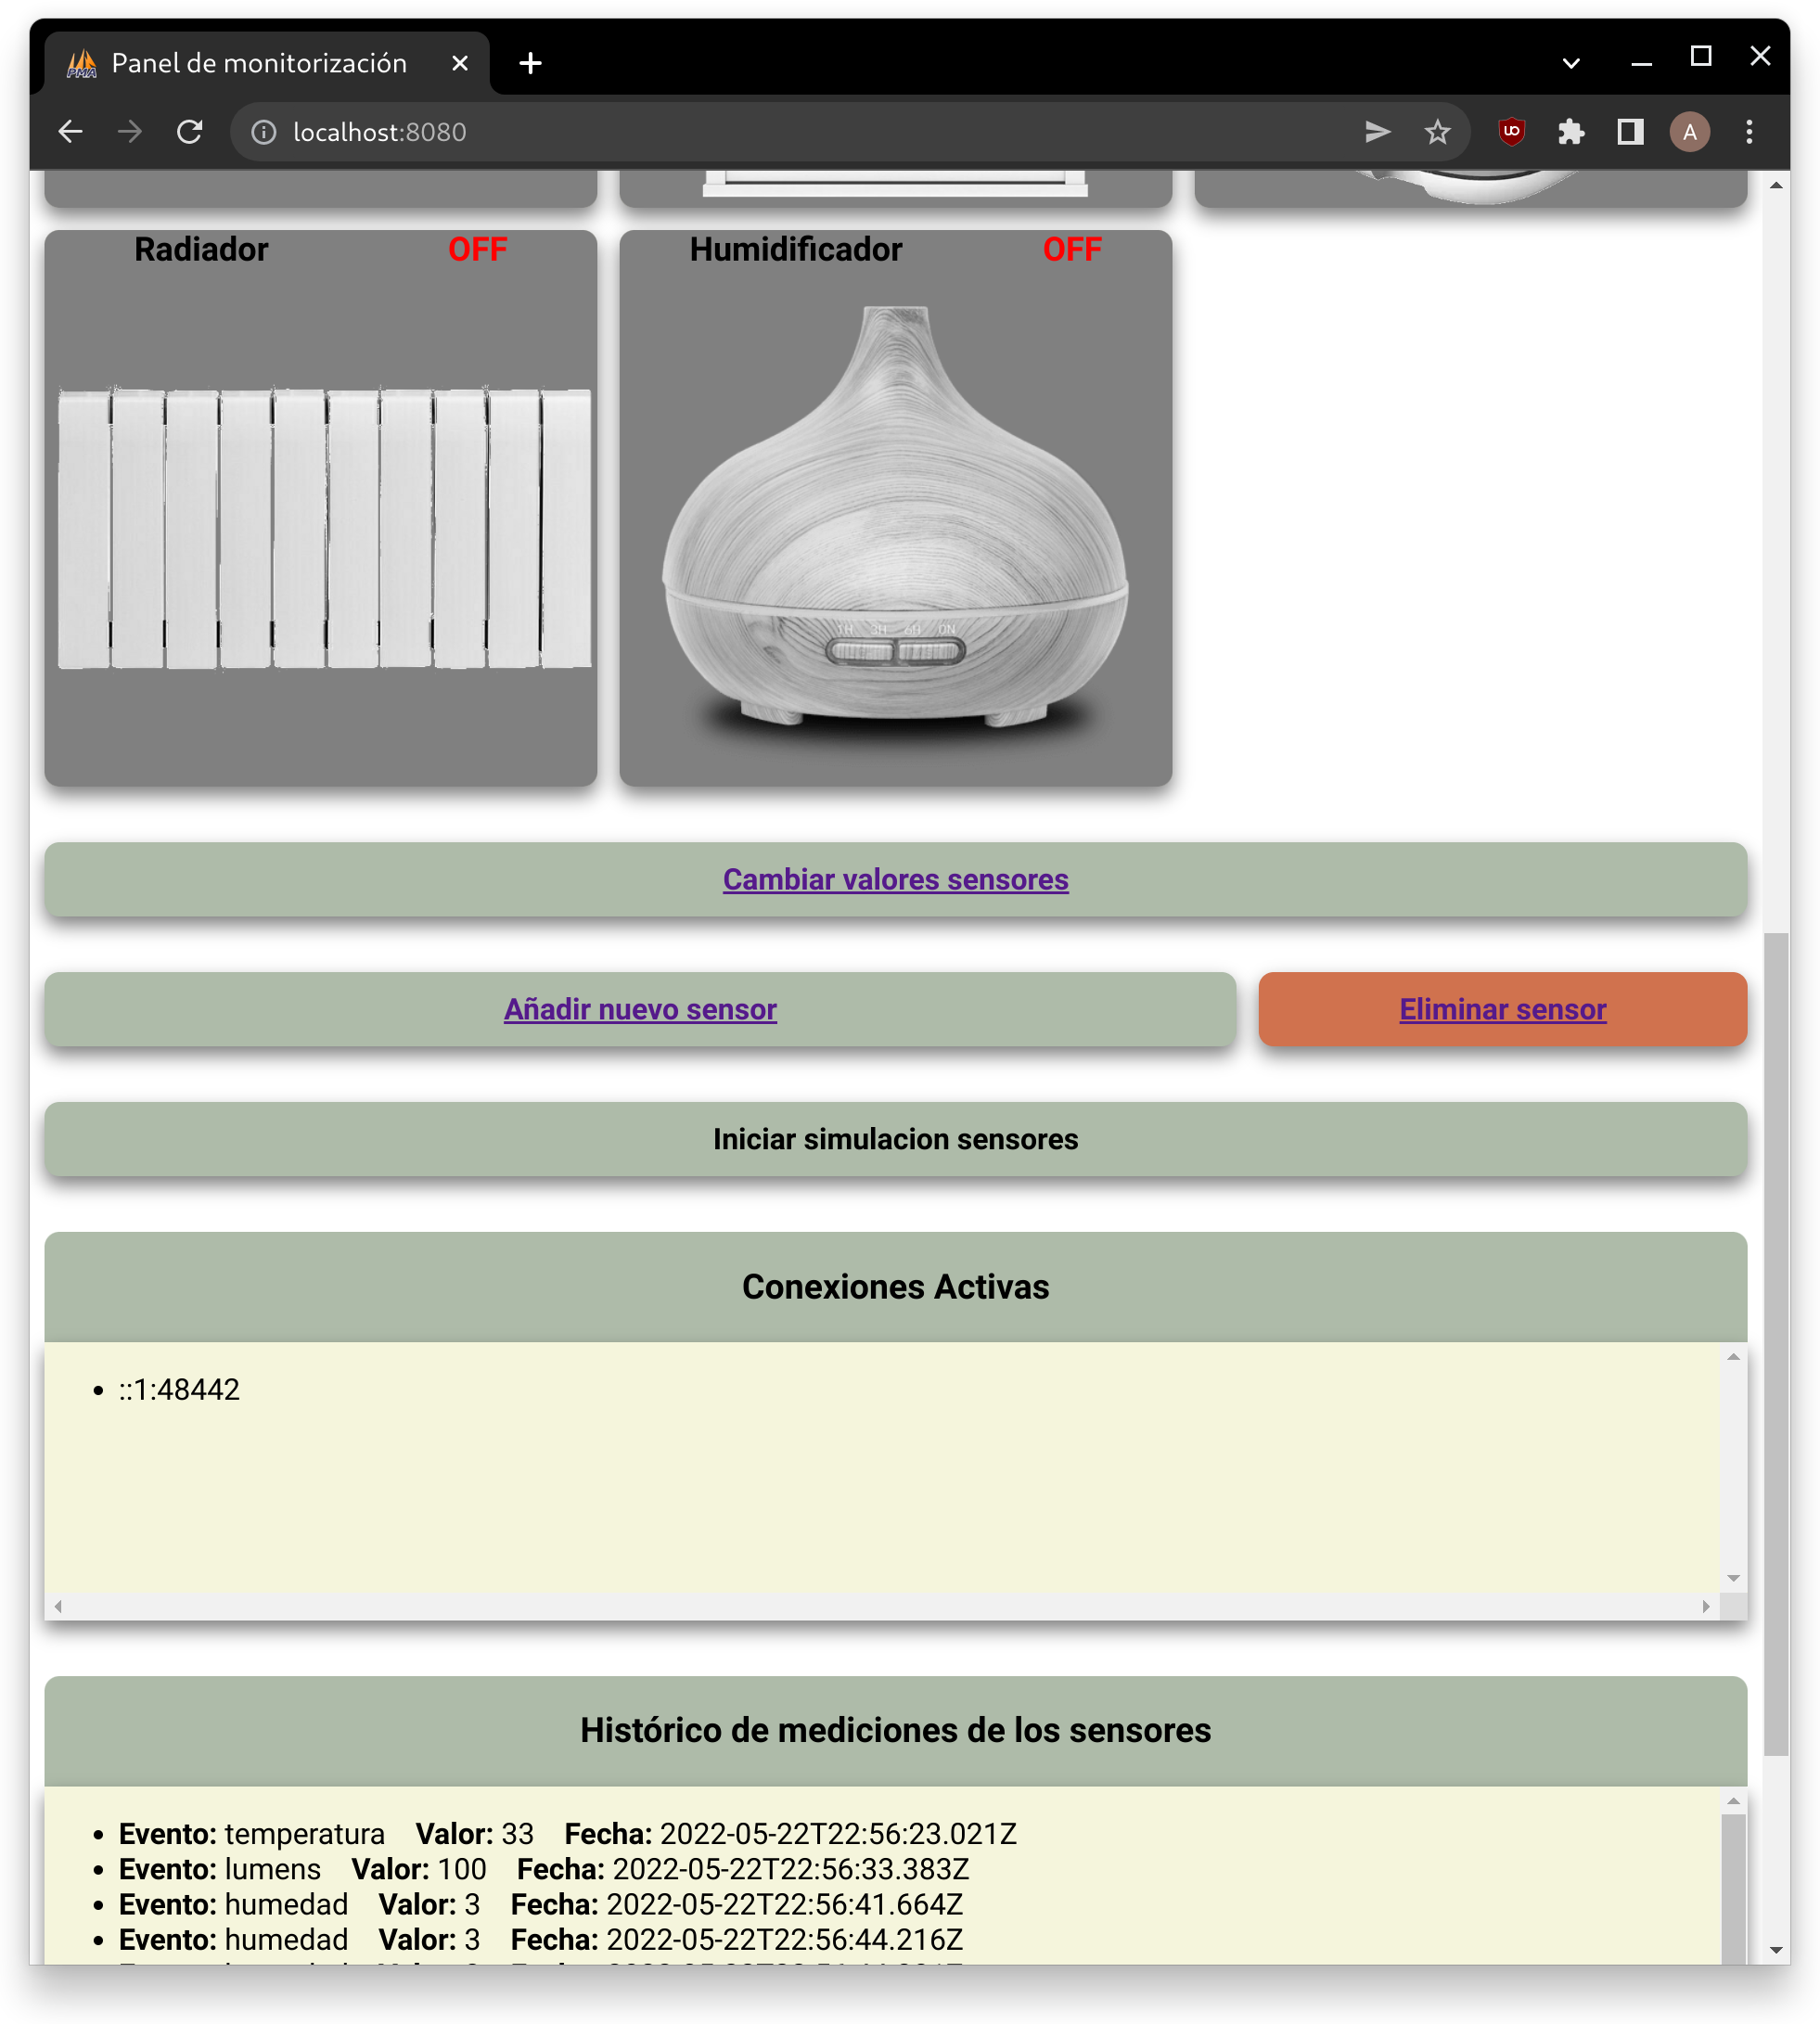
\includegraphics[width=\textwidth]{images/pagina2.png}
    \end{minipage}
\end{figure}

\begin{figure}[H]
    \centering
    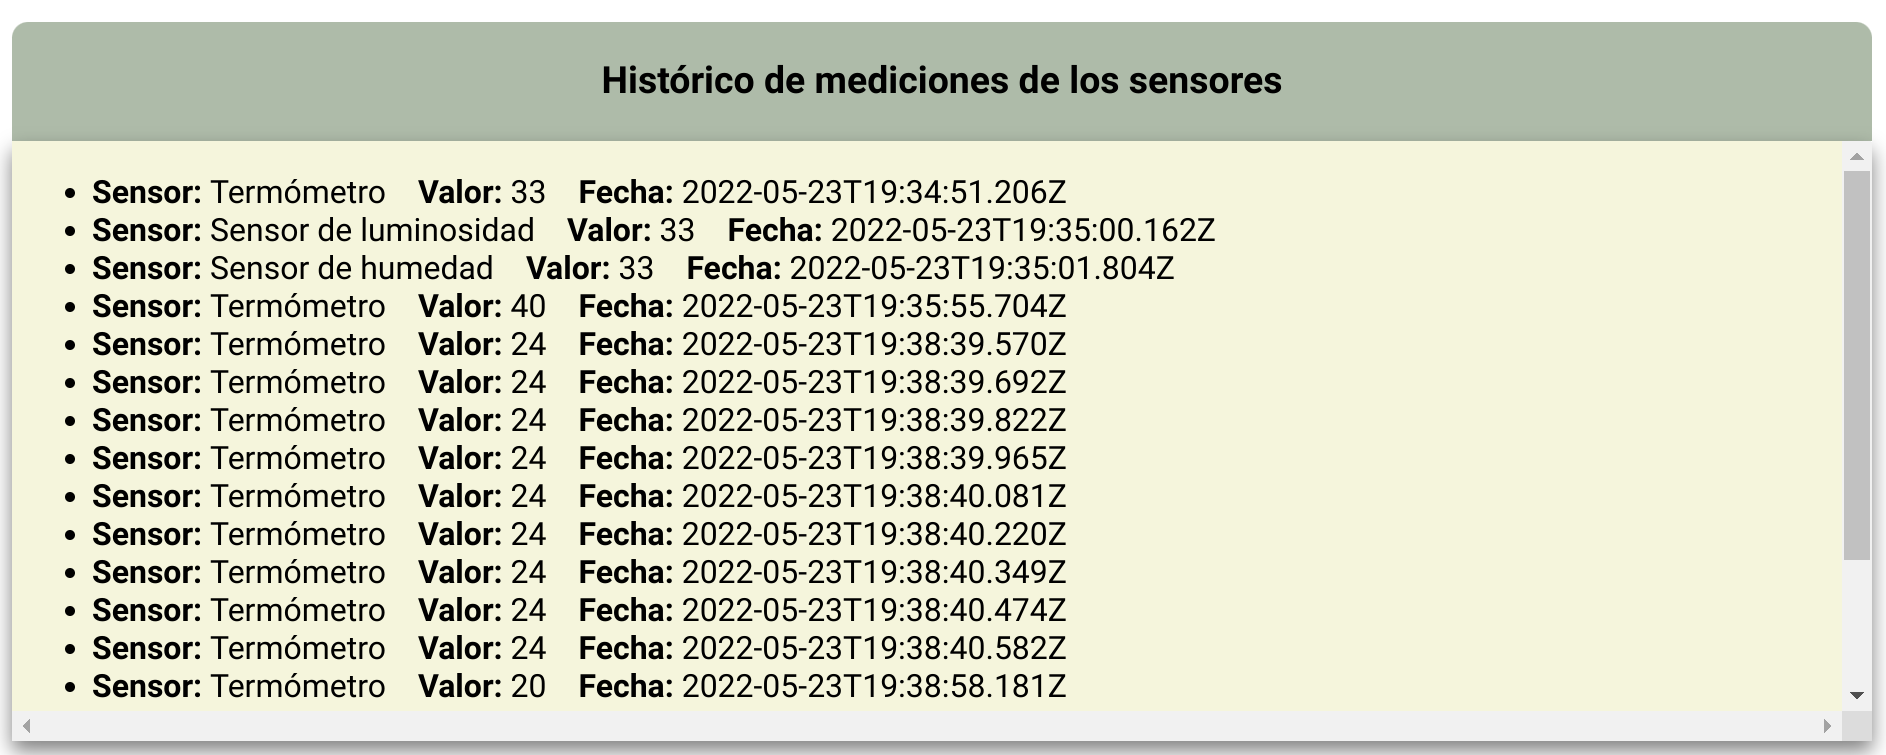
\includegraphics[width=0.7\textwidth]{images/pagina3.png}
\end{figure}

Como se puede ver, tienes otro sensor más y 3 actuadores más. Esto forma parte del extra, que explicare mas adelante. Ademas, si se pulsa en un actuador, este se activa o desactiva, reflejandose el cambio en los demas clientes conectados y en los que se van a conectar.

\begin{figure}[H]
    \centering
    \begin{minipage}[H]{0.49\textwidth}
        \centering
        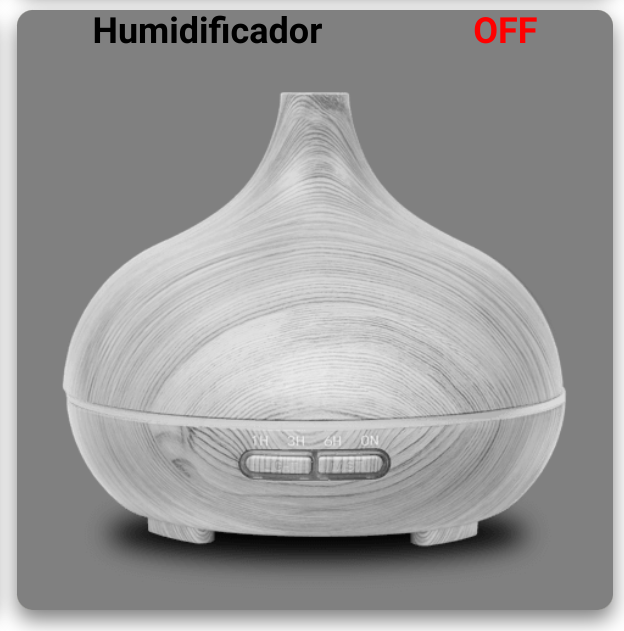
\includegraphics[width=\textwidth]{images/humoff.png}
        \caption{Humidificador apagado.}
    \end{minipage}
    \hfill
    \begin{minipage}[H]{0.49\textwidth}
        \centering
        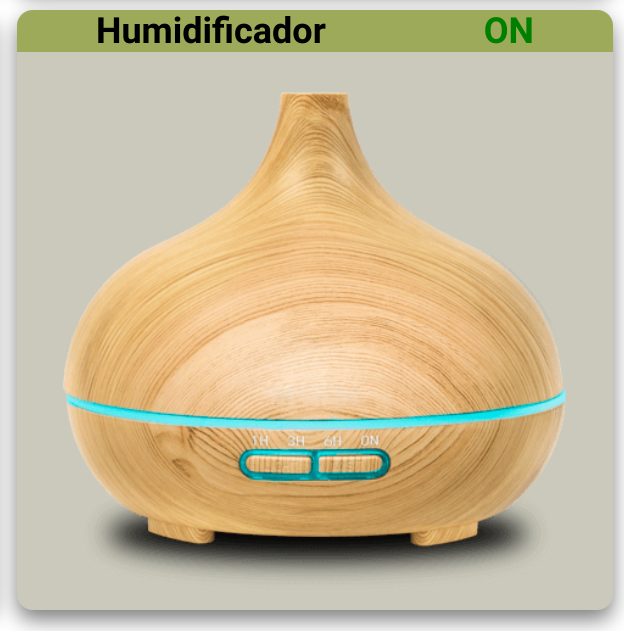
\includegraphics[width=\textwidth]{images/humon.png}
        \caption{Humidificador encendido}
    \end{minipage}
\end{figure}

Tambien se puede observar que abajo tiene la opcion de cambiar los valores de los sensores. Cuando se pulsa lleva a una pagina distinta con un formulario para cambiar el valor del sensor elegido en el desplegable:

%MOSTRAR FOTO DEL FORMULARIO
\begin{figure}[H]
    \centering
    
\includegraphics[width=0.7\textwidth]{images/cambiarsensor.png}
    \caption{Boton para cambiar los valores de los sensores.}
\end{figure}

Un problema que tuve era que qería que al enviar el nuevo valor del sensor, se redireccionase a la pagina principal de nuevo, pero el emit que realizaba el socket no se llegaba a mandar al servidor, haciendo que los cambios no se produjesen. Al final opte por no redireccionar a ninguna pagina, esto hizo que ya funcionase, ademas asi se permite modificar el valor de varios sensores a la vez. Cabe decir que cuando se envia el valor nuevo, este se guarda en la base de datos y se muestra en la pagina principal de todos los clientes que se encuentren en la misma.

%MOSTRAR FOTO DE UN CAMBIO, LUEGO DE LA PAGINA PRINCIPAL CON EL CAMBIO DEL SENSOR Y FINALMENTE OTRA CON EL CAMBIO REFLEJADO EN LA BASE DE DATOS.
\begin{figure}[H]
    \centering
    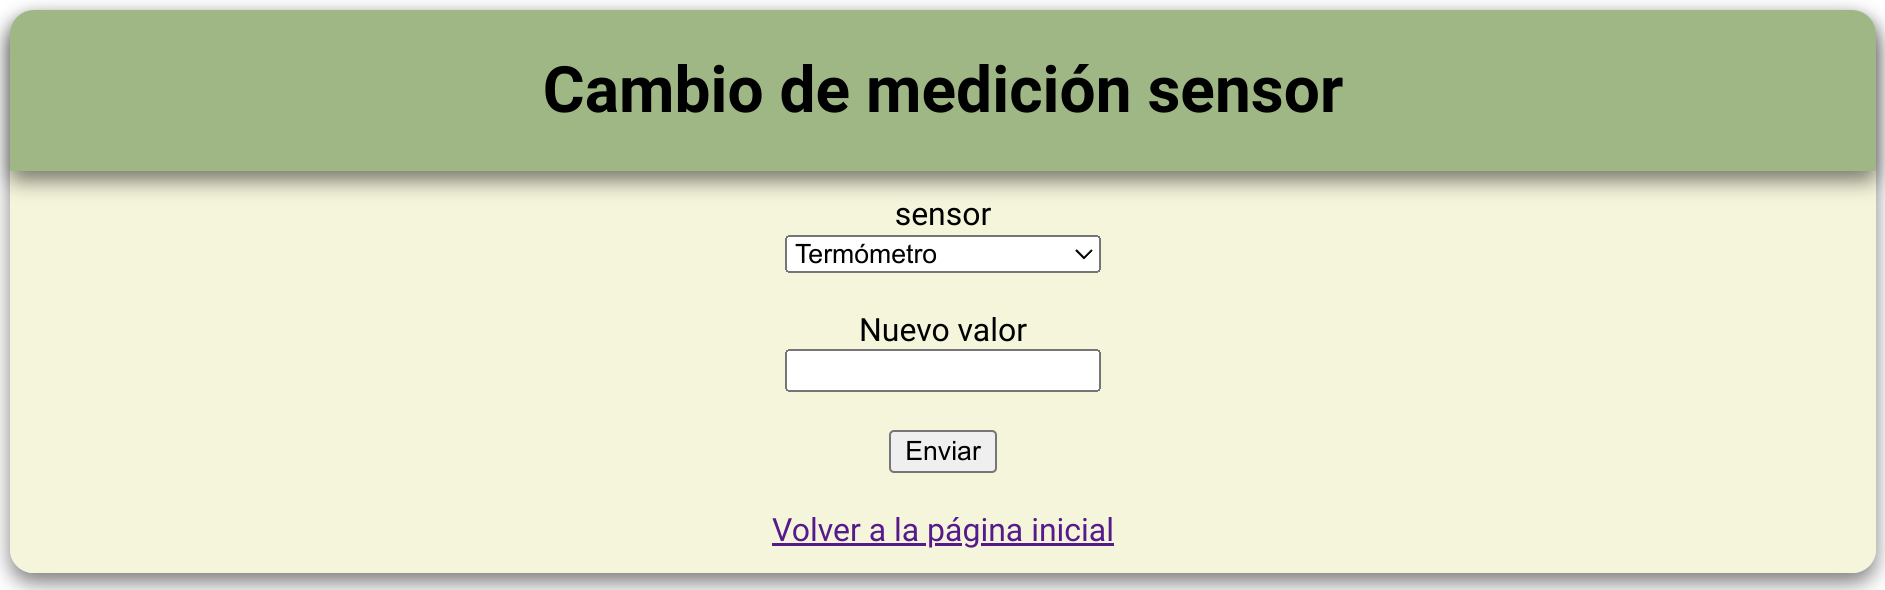
\includegraphics[width=0.7\textwidth]{images/form.png}
    \caption{Formulario para cambiar el valor del sensor.}
\end{figure}

\begin{figure}[H]
    \centering
    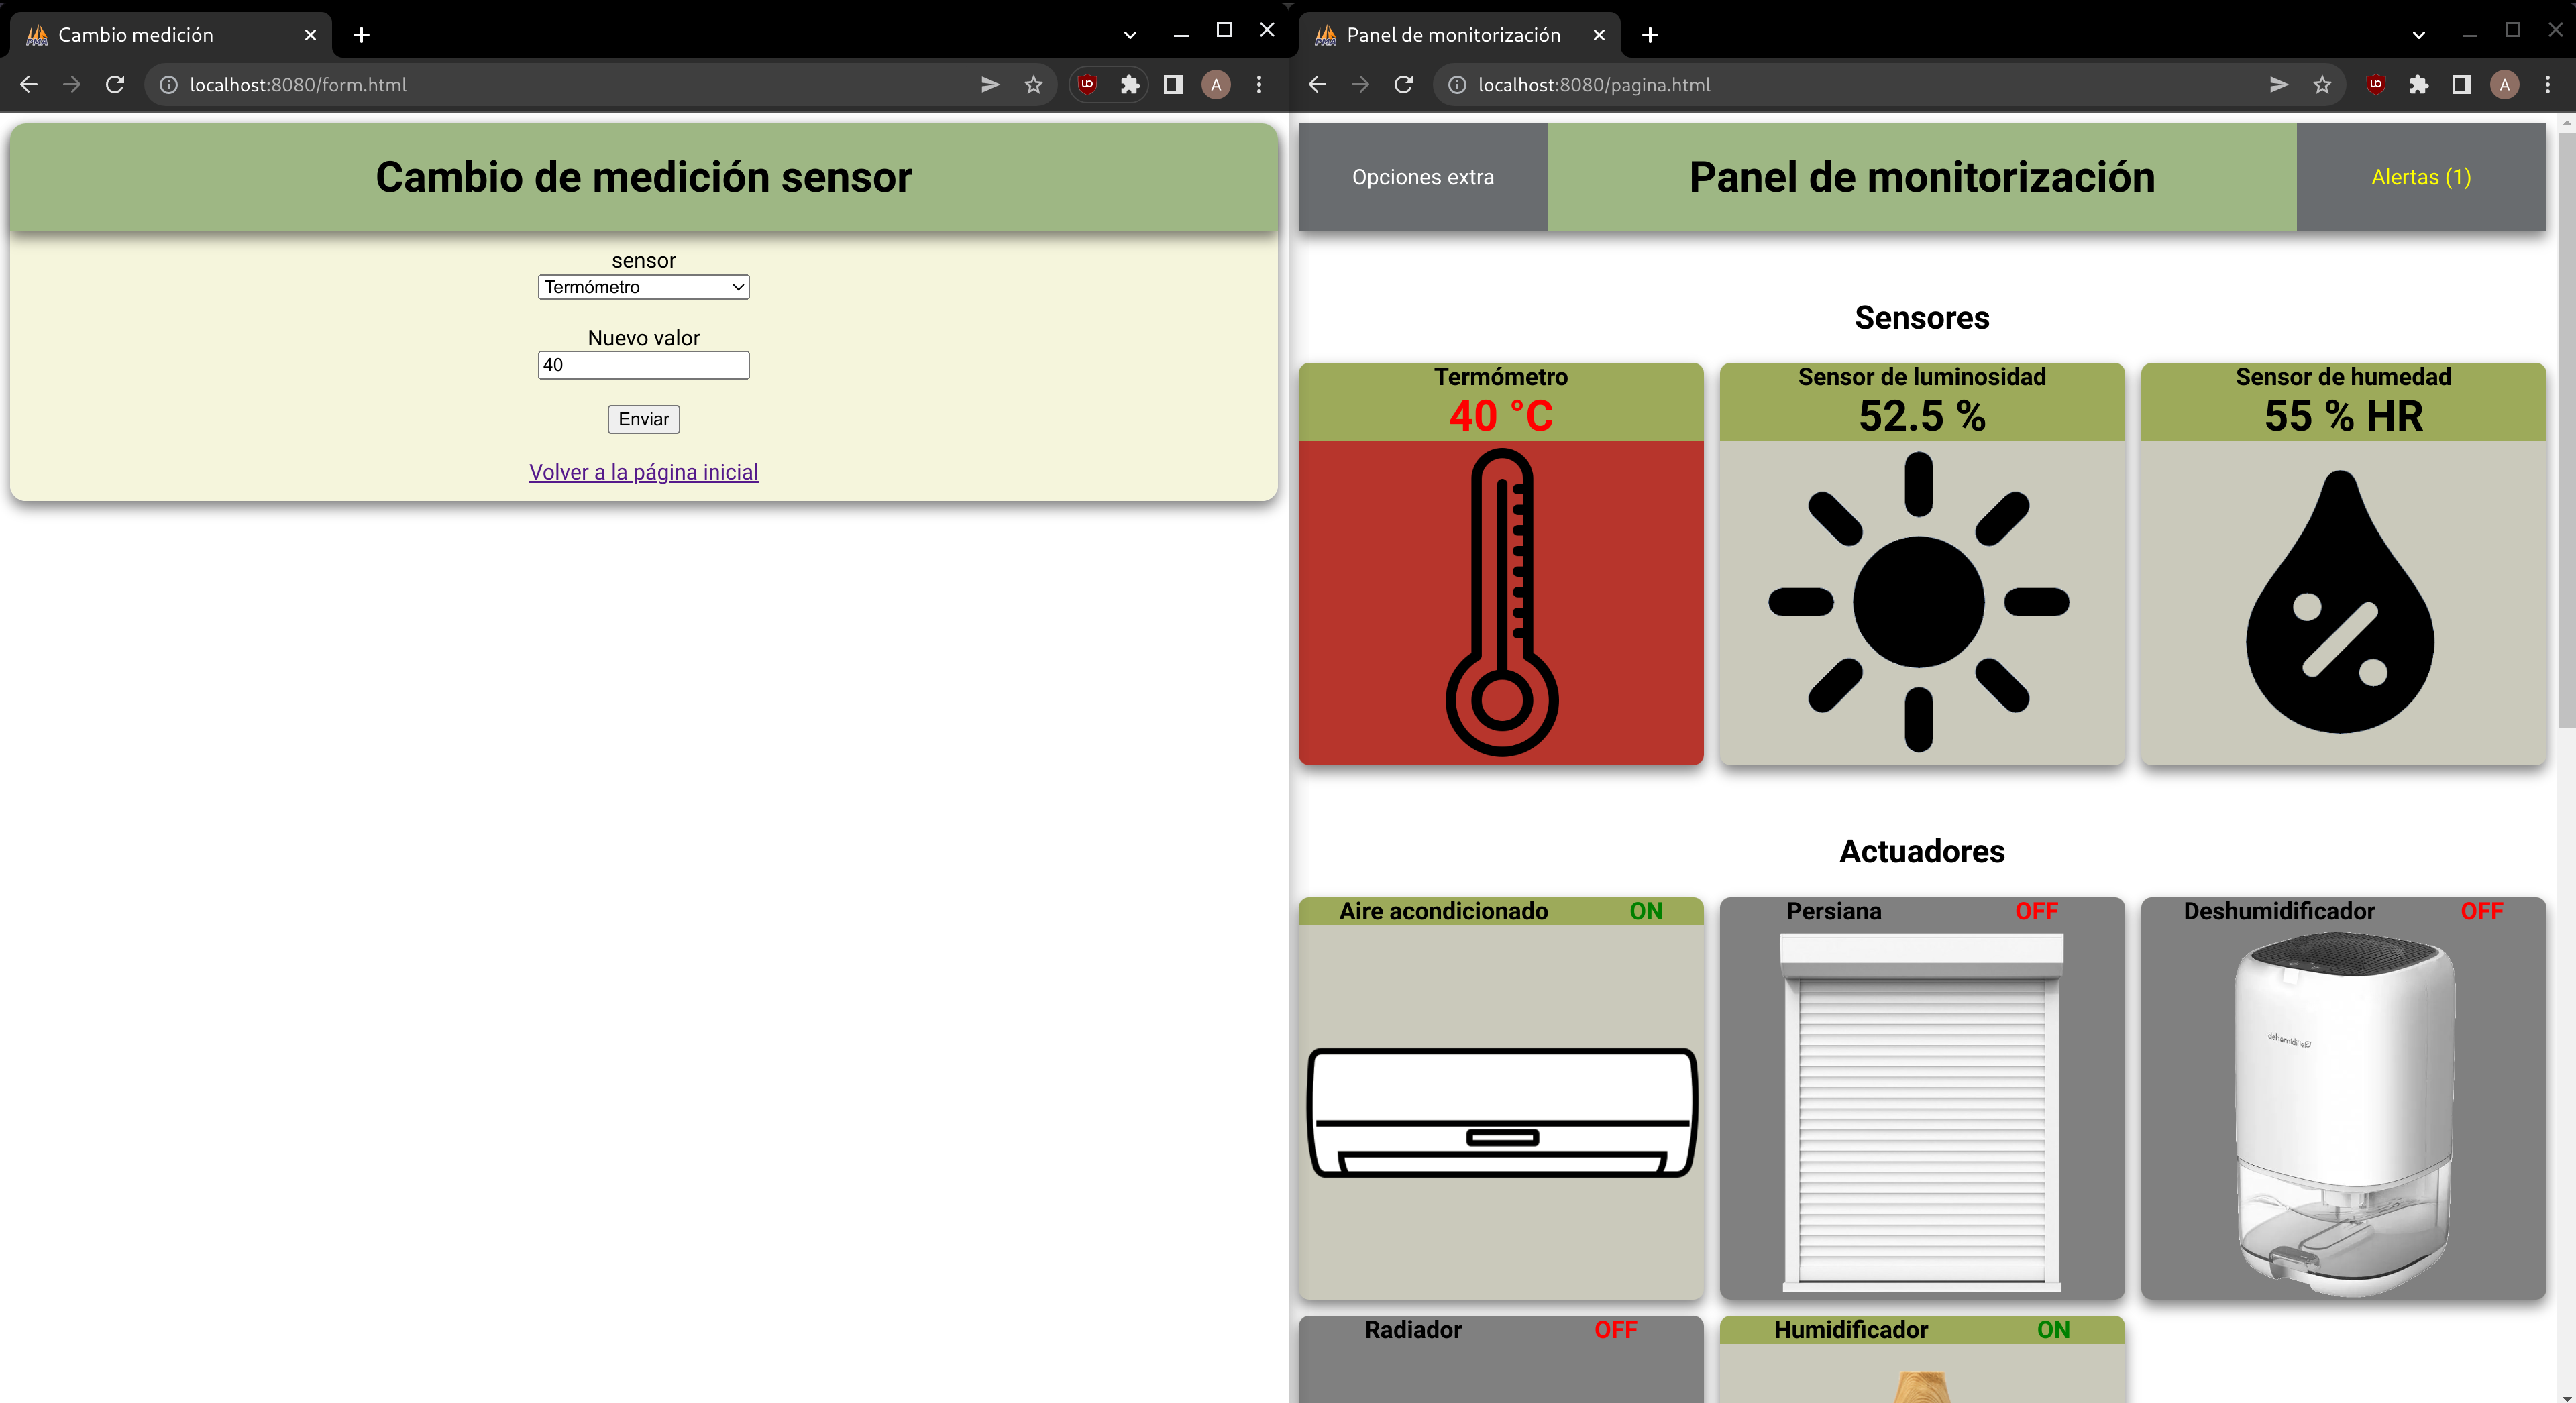
\includegraphics[width=0.7\textwidth]{images/cambiotemp.png}
    \caption{Cambio del sensor de temperatura}
\end{figure}

\begin{figure}[H]
    \centering
    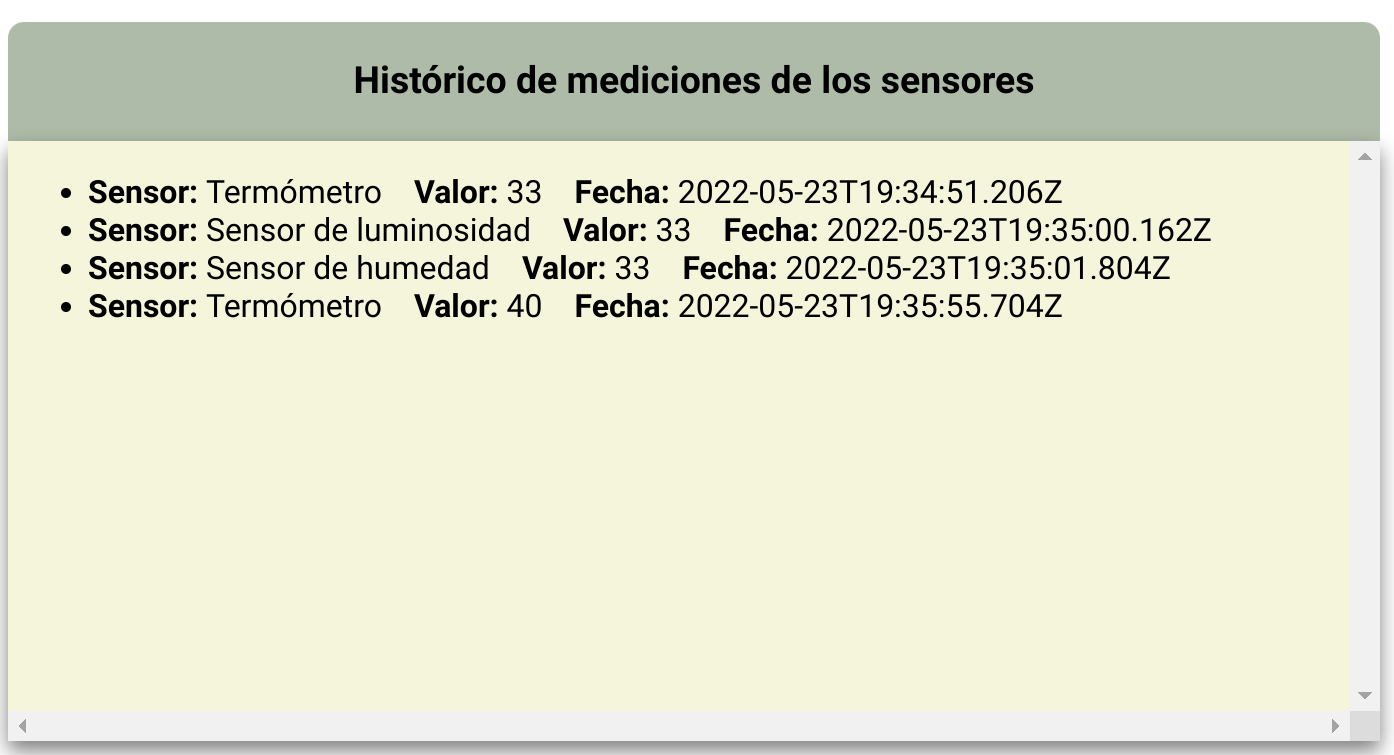
\includegraphics[width=0.7\textwidth]{images/cambiovalordb.png}
    \caption{Cambio reflejado en la pagina y en la base de datos.}
\end{figure}


POr ultimo, se puede observar que arriba a la derecha hay una opcion de alertas. Estas se activan (para la parte obligatoria, por ahora) cuando los sensores detectan un valor maximo o minimo. Cuando aparece un numero mayor que 0 significa que hay alguna alerta, y ademas, si se pulsa en el texto o en el recuadro, aparece un desplegable con todas las alertas mas detalladas.

\begin{figure}[H]
    \centering
    \begin{minipage}[H]{0.49\textwidth}
        \centering
        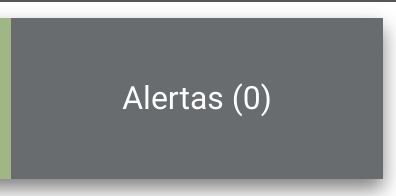
\includegraphics[width=\textwidth]{images/alerta0.png}
        \caption{Ninguna alerta.}
    \end{minipage}
    \hfill
    \begin{minipage}[H]{0.49\textwidth}
        \centering
        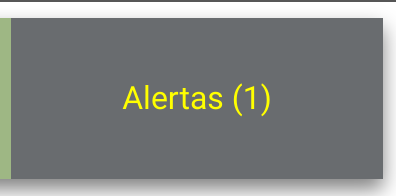
\includegraphics[width=\textwidth]{images/alerta1.png}
        \caption{Hay una alerta}
    \end{minipage}
\end{figure}

\begin{figure}[H]
    \centering
    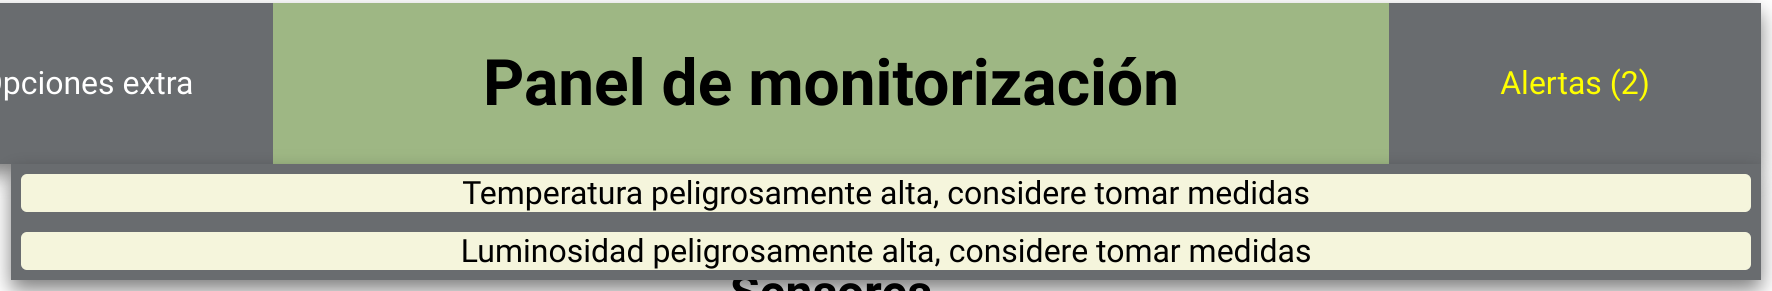
\includegraphics[width=0.7\textwidth]{images/alertamsg.png}
    \caption{Explicación de las alertas.}
\end{figure}

Ahora bien, he intentado generalizar lo maximo posible los sensores para que los eventos correspondientes puedan ser compartidos por todos y se simplifique la insercion de nuevos sensores en el futuro. Para ello, he creado un JSON con toda la informacion relativa de un sensor. Este a su vez se almacena en un array. El JSON tiene los siguientes campos:

\begin{itemize}
    \item \textbf{id: }Identificador del sensor.
    \item \textbf{name: }Nombre que se va a usar para las etiquetas HTML correspondientes a dicho sensor y poder direccionarlo en JavaScript.
    \item \textbf{sensorName: }Nombre del sensor que aparecera en la pantalla principal.
    \item \textbf{unit: }Unidades usadas por el sensor.
    \item \textbf{maxWarningMsg: }Mensaje de alerta que se muestra cuando se llegue a ``highWarningValue''.
    \item \textbf{highWarningValue: }Valor superior a partir del cual ya se muestra una alerta.
    \item \textbf{redValue: }Valor límite que el usuario decide. Si se llega a este valor, el sistema tomará la decisión de accionar el actuador correspondiente.
    \item \textbf{maxValue: }Valor máximo que el sensor puede soportar.
    \item \textbf{minWarningMsg: }Mensaje de alerta que se muestra cuando se llegue a ``lowWarningValue''.
    \item \textbf{lowWarningValue: }Valor inferior a partir del cual ya se muestra una alerta.
    \item \textbf{blueValue: }Valor inferior limite que el usuario decide. Si se llega a este valor, el sistema tomará la decision de accionar el actuador correspondiente.
    \item \textbf{minValue: }Valor minimo que el sensor puede soportar.
    \item \textbf{imageDir: }Directorio donde se encuentra la imagen que se va a insertar.
    \item \textbf{currentValue: }Valor actual del sensor.
\end{itemize}

%Si da tiempo poner un dibujo de esto

He realizado lo mismo para los actuadores, que si bien en la parte extra no se pueden crear mas, me ha parecido mas correcto que todos compartan el mismo evento y se haga de manera generica.

Los actuadores tienen los siguientes campos:

\begin{itemize}
    \item \textbf{id: }Identificador del actuador.
    \item \textbf{name: }Nombre del actuador.
    \item \textbf{state: }Estado actual del actuador.
    \item \textbf{idName: }Identificador que se usa para direccionar en JavaScript.
    \item \textbf{img: }Ruta de la imagen que se va a usar.
\end{itemize}

Los eventos que se usan para la página principal son los siguientes:

\begin{itemize}
    \item \textbf{clientes: }Obtiene la lista de los clientes conectados en cada momentos. Se actualiza cada vez que se conecta o desconecta algun cliente.
    \item \textbf{obtener-sensores: }Sirve para inicializar la pantalla con todos los sensores que hay en el sistema. También es accionado en el cliente cuando se añade o elimina un sensor.
    \item \textbf{cambio-sensor: }Se acciona en el cliente cuando se cambia el valor de un sensor para cambiarle el estilo si está en zona de alerta. Mientras que en el servidor se acciona cuando se envía el nuevo valor a través del formulario.
    \item \textbf{historial: }Actualiza la información del historial de cambios de los valores en los sensores. En el servidor se acciona cuando un cliente nuevo se conecta.
    \item \textbf{nuevo-registro: }Envia el nuevo registro que se ha producido al cambiar el valor de un sensor. Este evento extra permite una mayor eficiencia ya que no se deben mandar todos los registros y reconstruirlos. Además evita ralentizaciones de MongoDB.
    \item \textbf{alerta: }Actualiza las alertas actuales. Cabe destacar que este evento no se puede hacer más eficiente (es decir, mandando solo la informacion necesaria como pasaba con el historial de registros de la base de datos), ya que pueden eliminarse valores intermedios del array en el servidor.
    \item \textbf{obtener-actuadores: }Al igual que ``obtener-sensores'', sirve para obtener todos los actuadores disponibles en la página.
    \item \textbf{cambio-actuador: }Actualiza el estado del actuador cuando otro cliente lo activa/desactiva.
\end{itemize}

No están explicados todos, ya que los demás son extra y los explicaré en la siguiente subsección.

Cuando un cliente se conecta, el servidor le manda todos los sensores, los actuadores, el historial, las alertas y los clientes conectados. Así se asegura que tenga la misma información que otros clientes.

%INTENTAR HACER UN DIAGRAMA PARA LA PAGINA PRINICIPAL


Para la parte del formulario de cambiar el valor de los sensores se hace uso del evento ``obtener-sensores'' para obtener los nombres de los sensores disponibles y mostrarlos en el desplegable y de ``obtener-sensor'', que se acciona cuando se envia la eleccion al servidor. Este a su vez emite mediante el evento ``cambio-sensor'' la información actualizada para que todos los clientes lo actualicen.

Por último, se pedia que cuando la temperatura y la luminosidad llegasen a un valor umbral, se cerrase la ventana. En mi caso lo que he hecho ha sido que cuando se llegue a cualquiera de los dos umbrales, se cierre la ventana, se accione el aire acondicionado y se apague el radiador.

%MOSTRAR UNA FOTO SOBRE ESTO CUANDO SE CAMBIA EL VALOR DE LUMINOSIDAD
\begin{figure}[H]
    \centering
    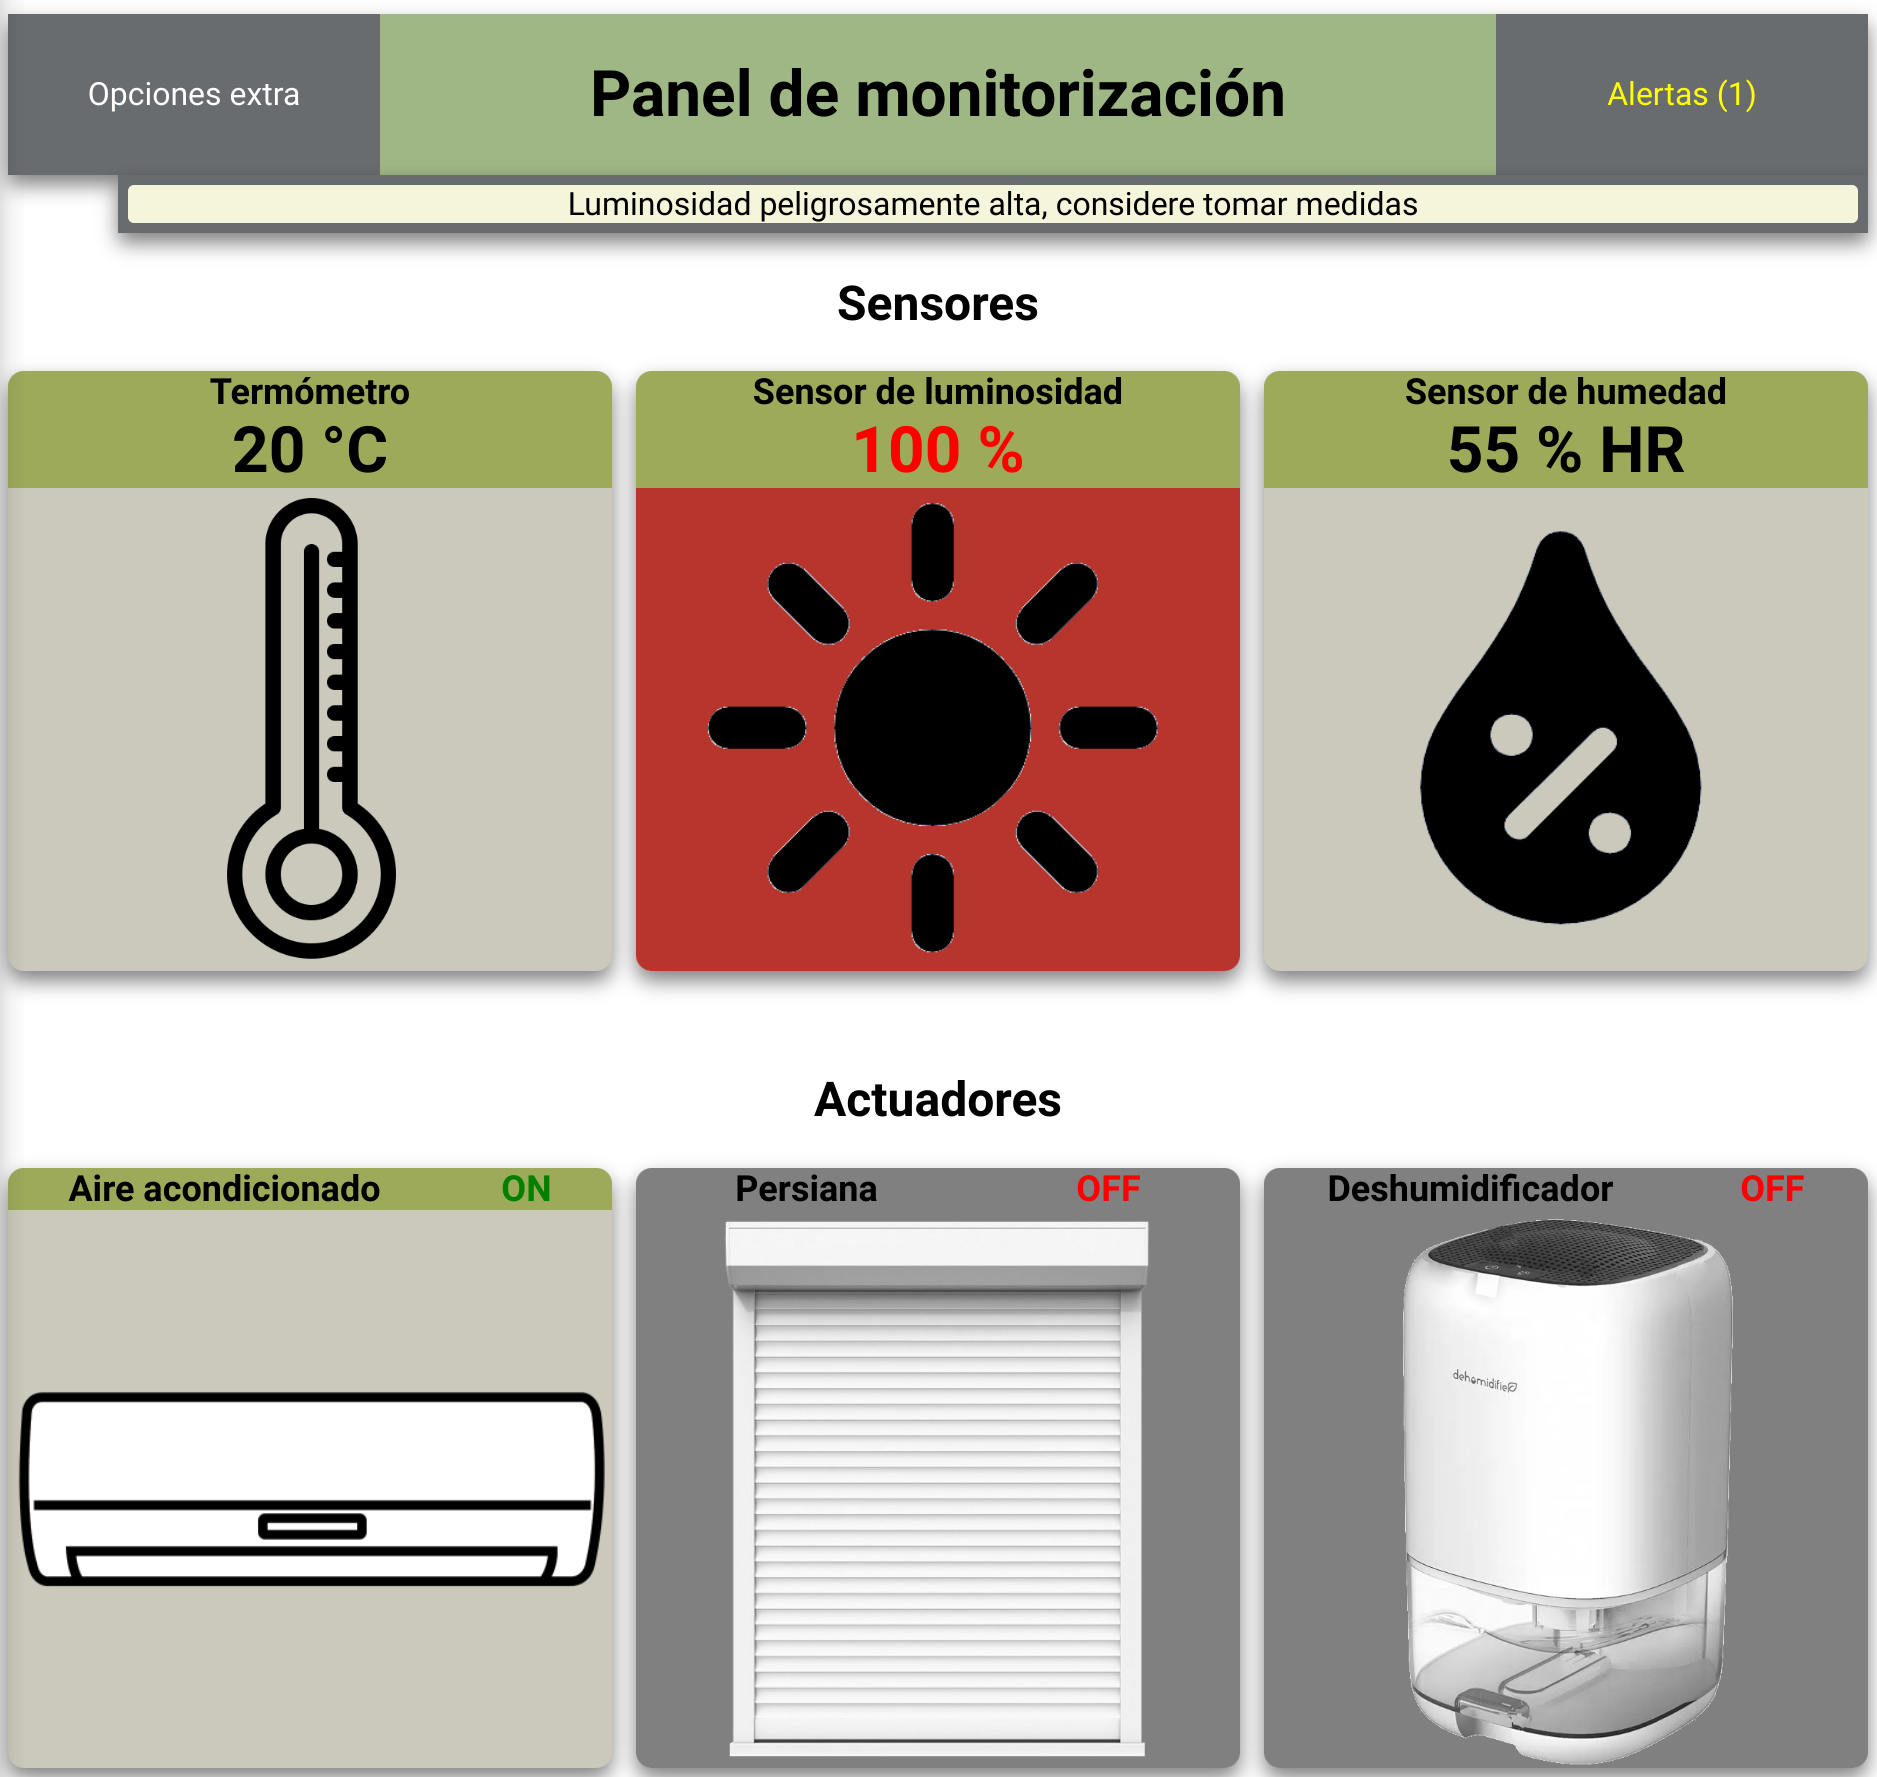
\includegraphics[width=0.7\textwidth]{images/muchaluz.png}
    \caption{Se ha encendido el aire acondicionado y se ha cerrado la ventana/persiana.}
\end{figure}

\subsubsection{Parte extra}
Para la parte extra he realizado lo siguiente:

\begin{itemize}
    \item Otro sensor más y tres actuadores más.
    \item Opcion de añadir y/o eliminar sensores.
    \item Más alertas de los valores de los sensores y de combinaciones de actuadores poco eficientes (por ejemplo, aire acondicionado y radiador encendido).
    \item Una simulación básica de cambio de temperatura y humedad con el tiempo, haciendo que el sistema sea autoregulable.
    \item Un sistema de chat grupal con inicio de sesión y registro necesario. Cuidando especialmente cuestiones de seguridad.
    \item Una pizarra digital distribuida en la que todos los clientes pueden dibujar a la vez y pueden a su vez ver los cambios de los demás en tiempo real.
\end{itemize}

He añadido un sensor de humedad. Mientras que de actuadores he añadido un radiador, un humidificador y un deshumidificador. Además, he añadido más lógica para las combinaciones de actuadores. Por ejemplo, si se enciende el radiador y el aire acondicionado, salta una alerta recomendando una acción. O si se enciende el humidificador y deshumidificador también salta otra alerta.

En total he realizado 4 posibles combinaciones ineficientes distintas.

%MOSTRAR FOTO DE UN ENTRELAZAMIENTO DE ACTUADORES
\begin{figure}[H]
    \centering
    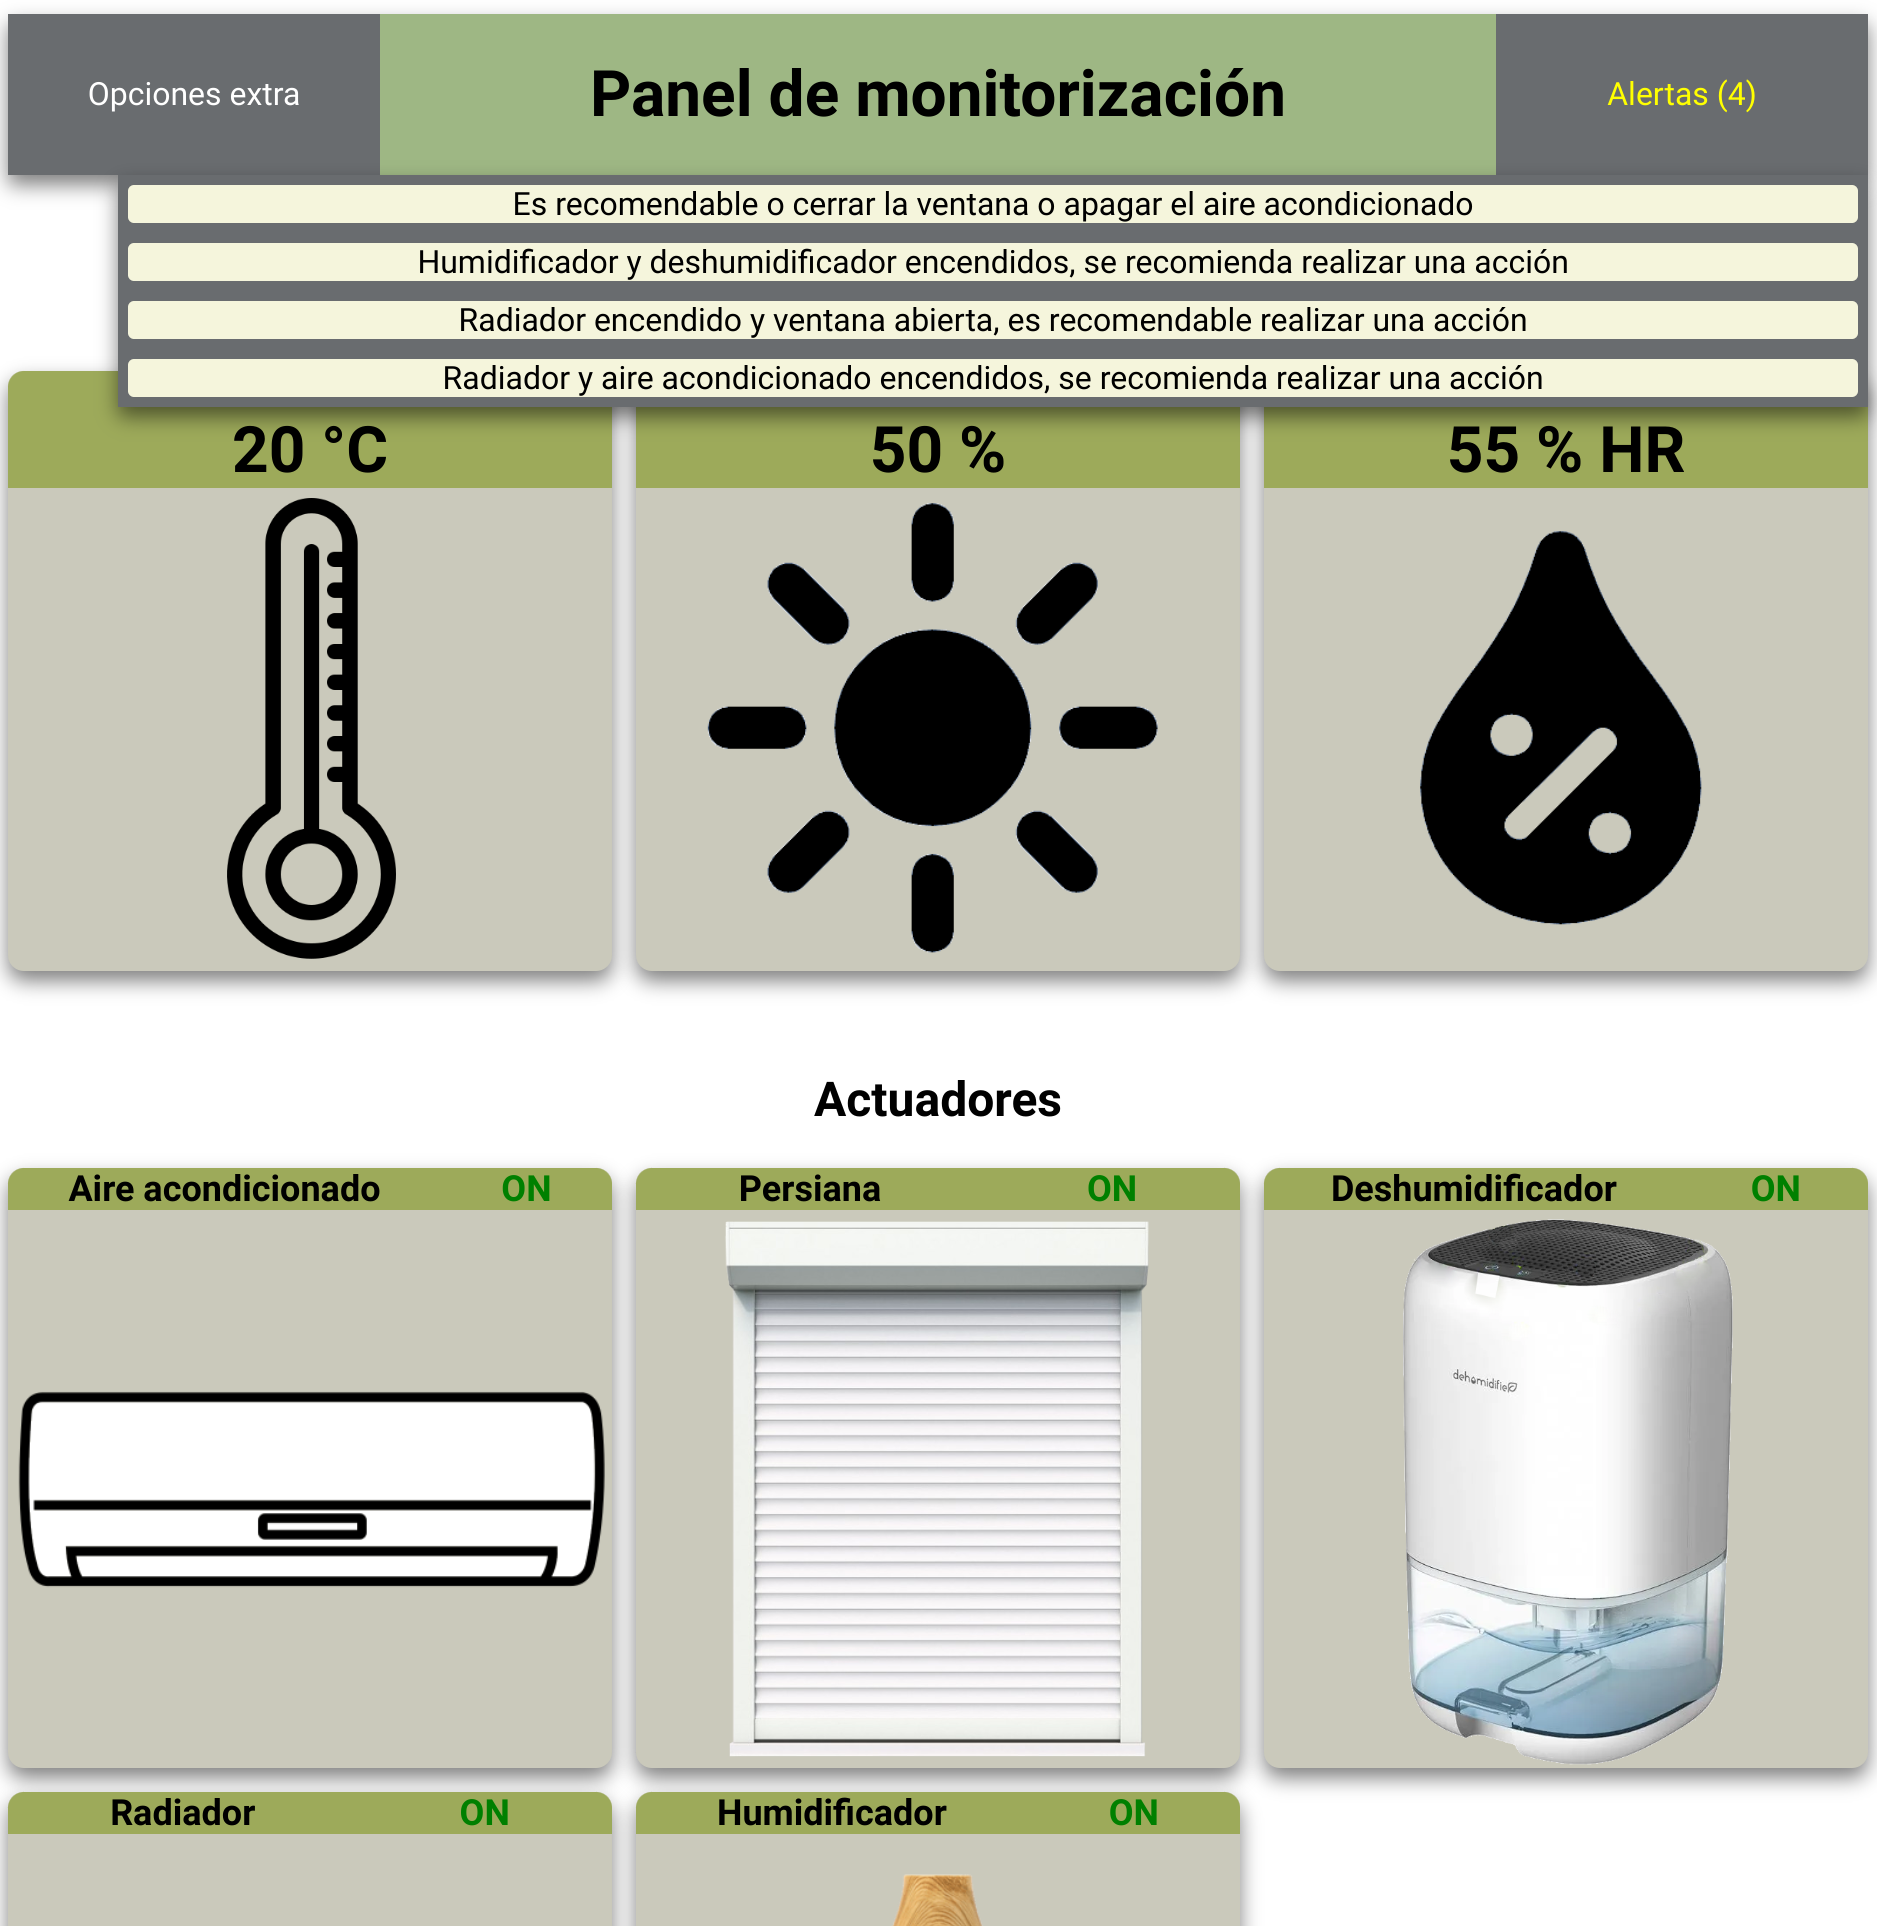
\includegraphics[width=0.7\textwidth]{images/actuadoresmal.png}
    \caption{Muestra alertas sore dispositivos encendidos.}
\end{figure}

Tambien he hecho un formulario con la posibilidad de añadir un nuevo sensor. Este formulario cuando se envia llama al evento ``add-sensor'' que envia el sensor al servidor, y este a su vez lo inserta en el array de sensores y mediante el evento ``obtener-sensores'' hace que se actualicen todos los clientes. 

%FOTO DE FORMULARIO PARA AÑADIR SENSOR
\begin{figure}[H]
    \centering
    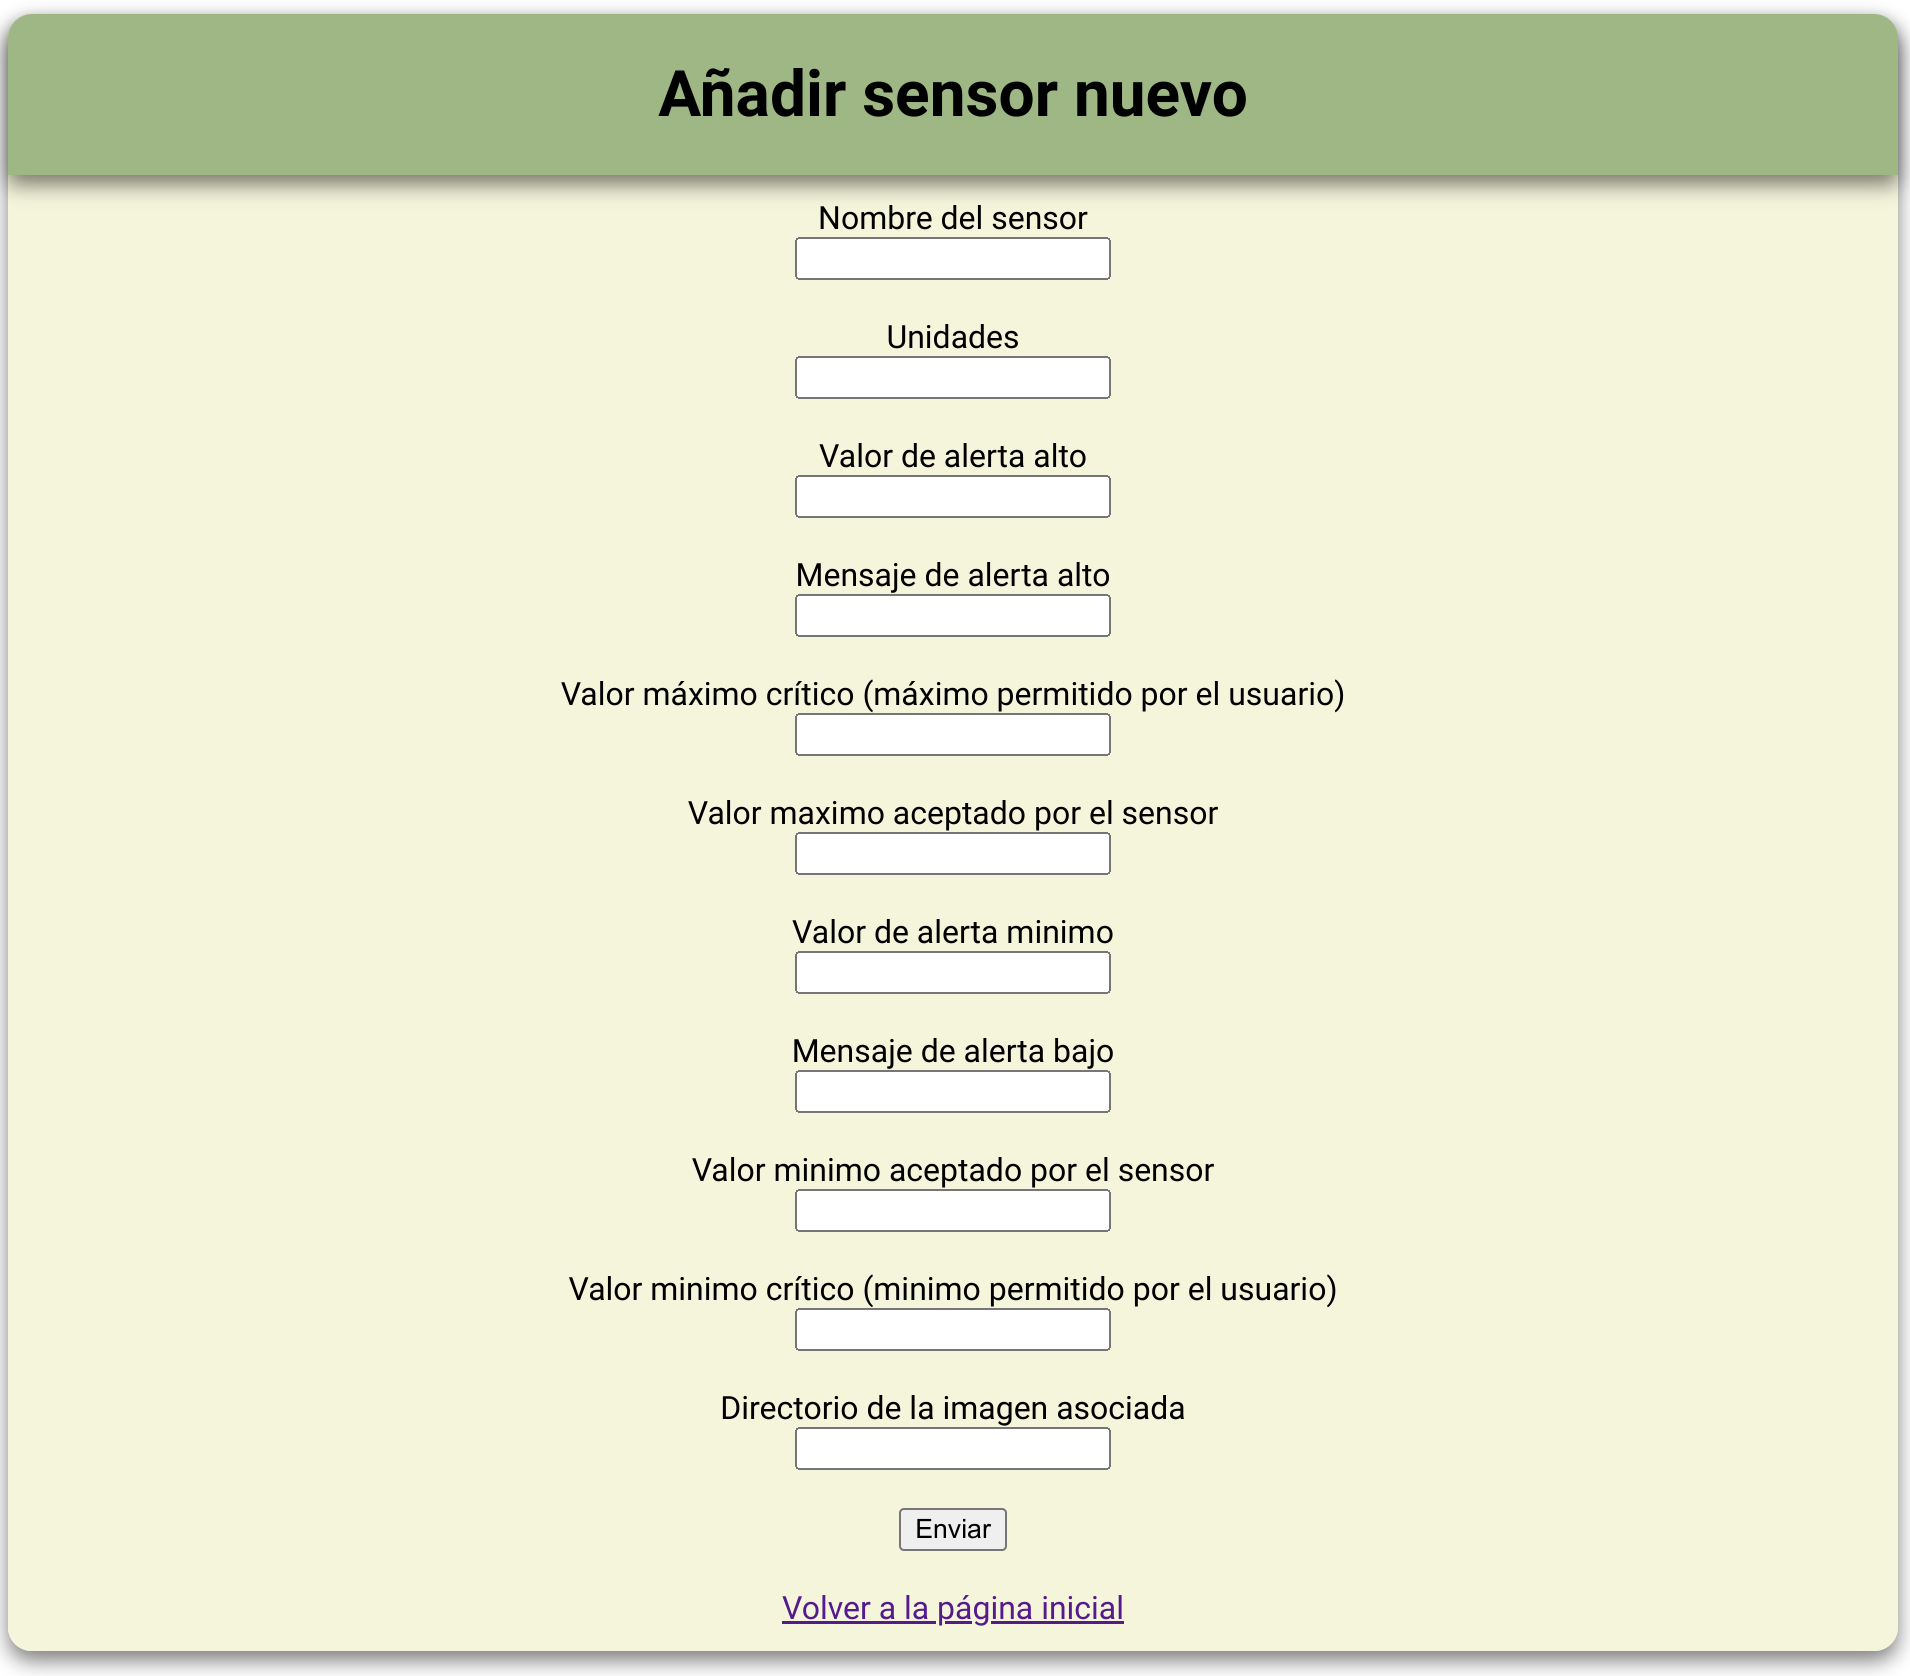
\includegraphics[width=0.7\textwidth]{images/addsensor.png}
    \caption{Formulario para añadir sensor.}
\end{figure}

La opción de eliminar sensor hace exactamente lo mismo, pero con el evento ``delete-sensor'', que elimina del array ese sensor en el servidor y tambien llama a ``obtener-sensores'' para actualizar a los demas clientes.

%FOTO DE FORMULARIO PARA ELIMINAR SENSOR
\begin{figure}[H]
    \centering
    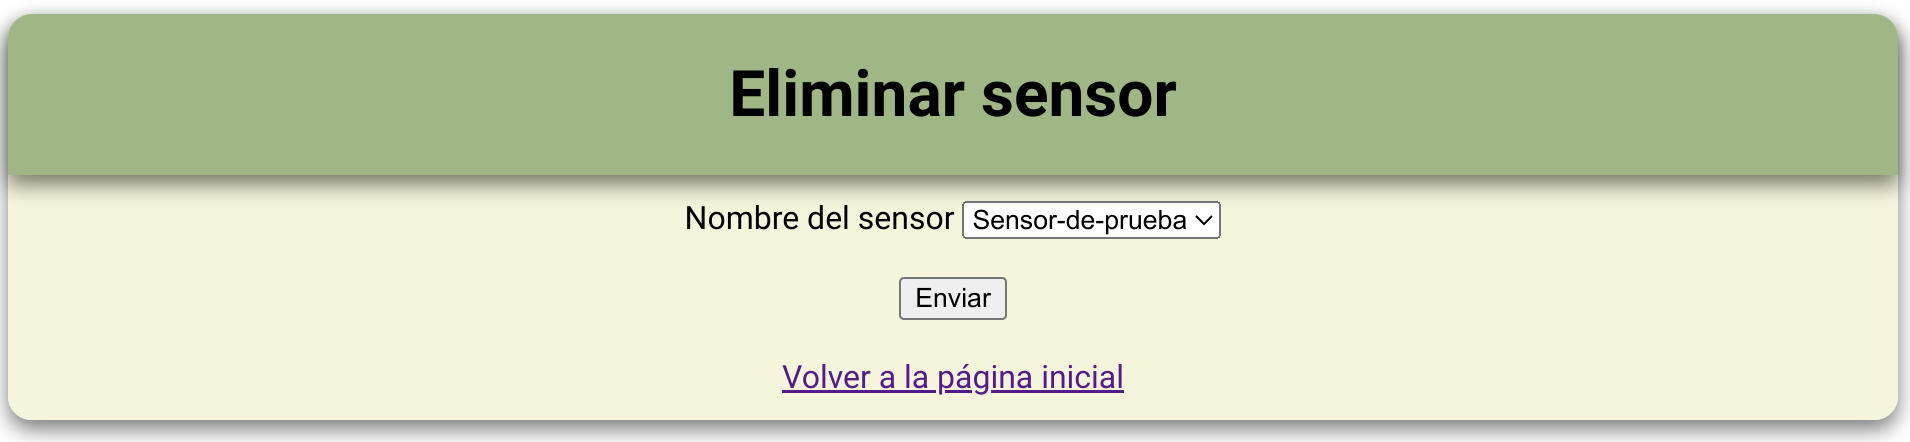
\includegraphics[width=0.7\textwidth]{images/deletesensorform.png}
    \caption{Formulario para eliminar un sensor.}
\end{figure}

Además, estos nuevos sensores tambien pueden lanzar alertas cuando se superen los valores umbrales con mensajes personalizados introducidos en el formulario.

%FOTO DE LA ALERTA DE UN SENSOR DE PRUEBA
\begin{figure}[H]
    \centering
    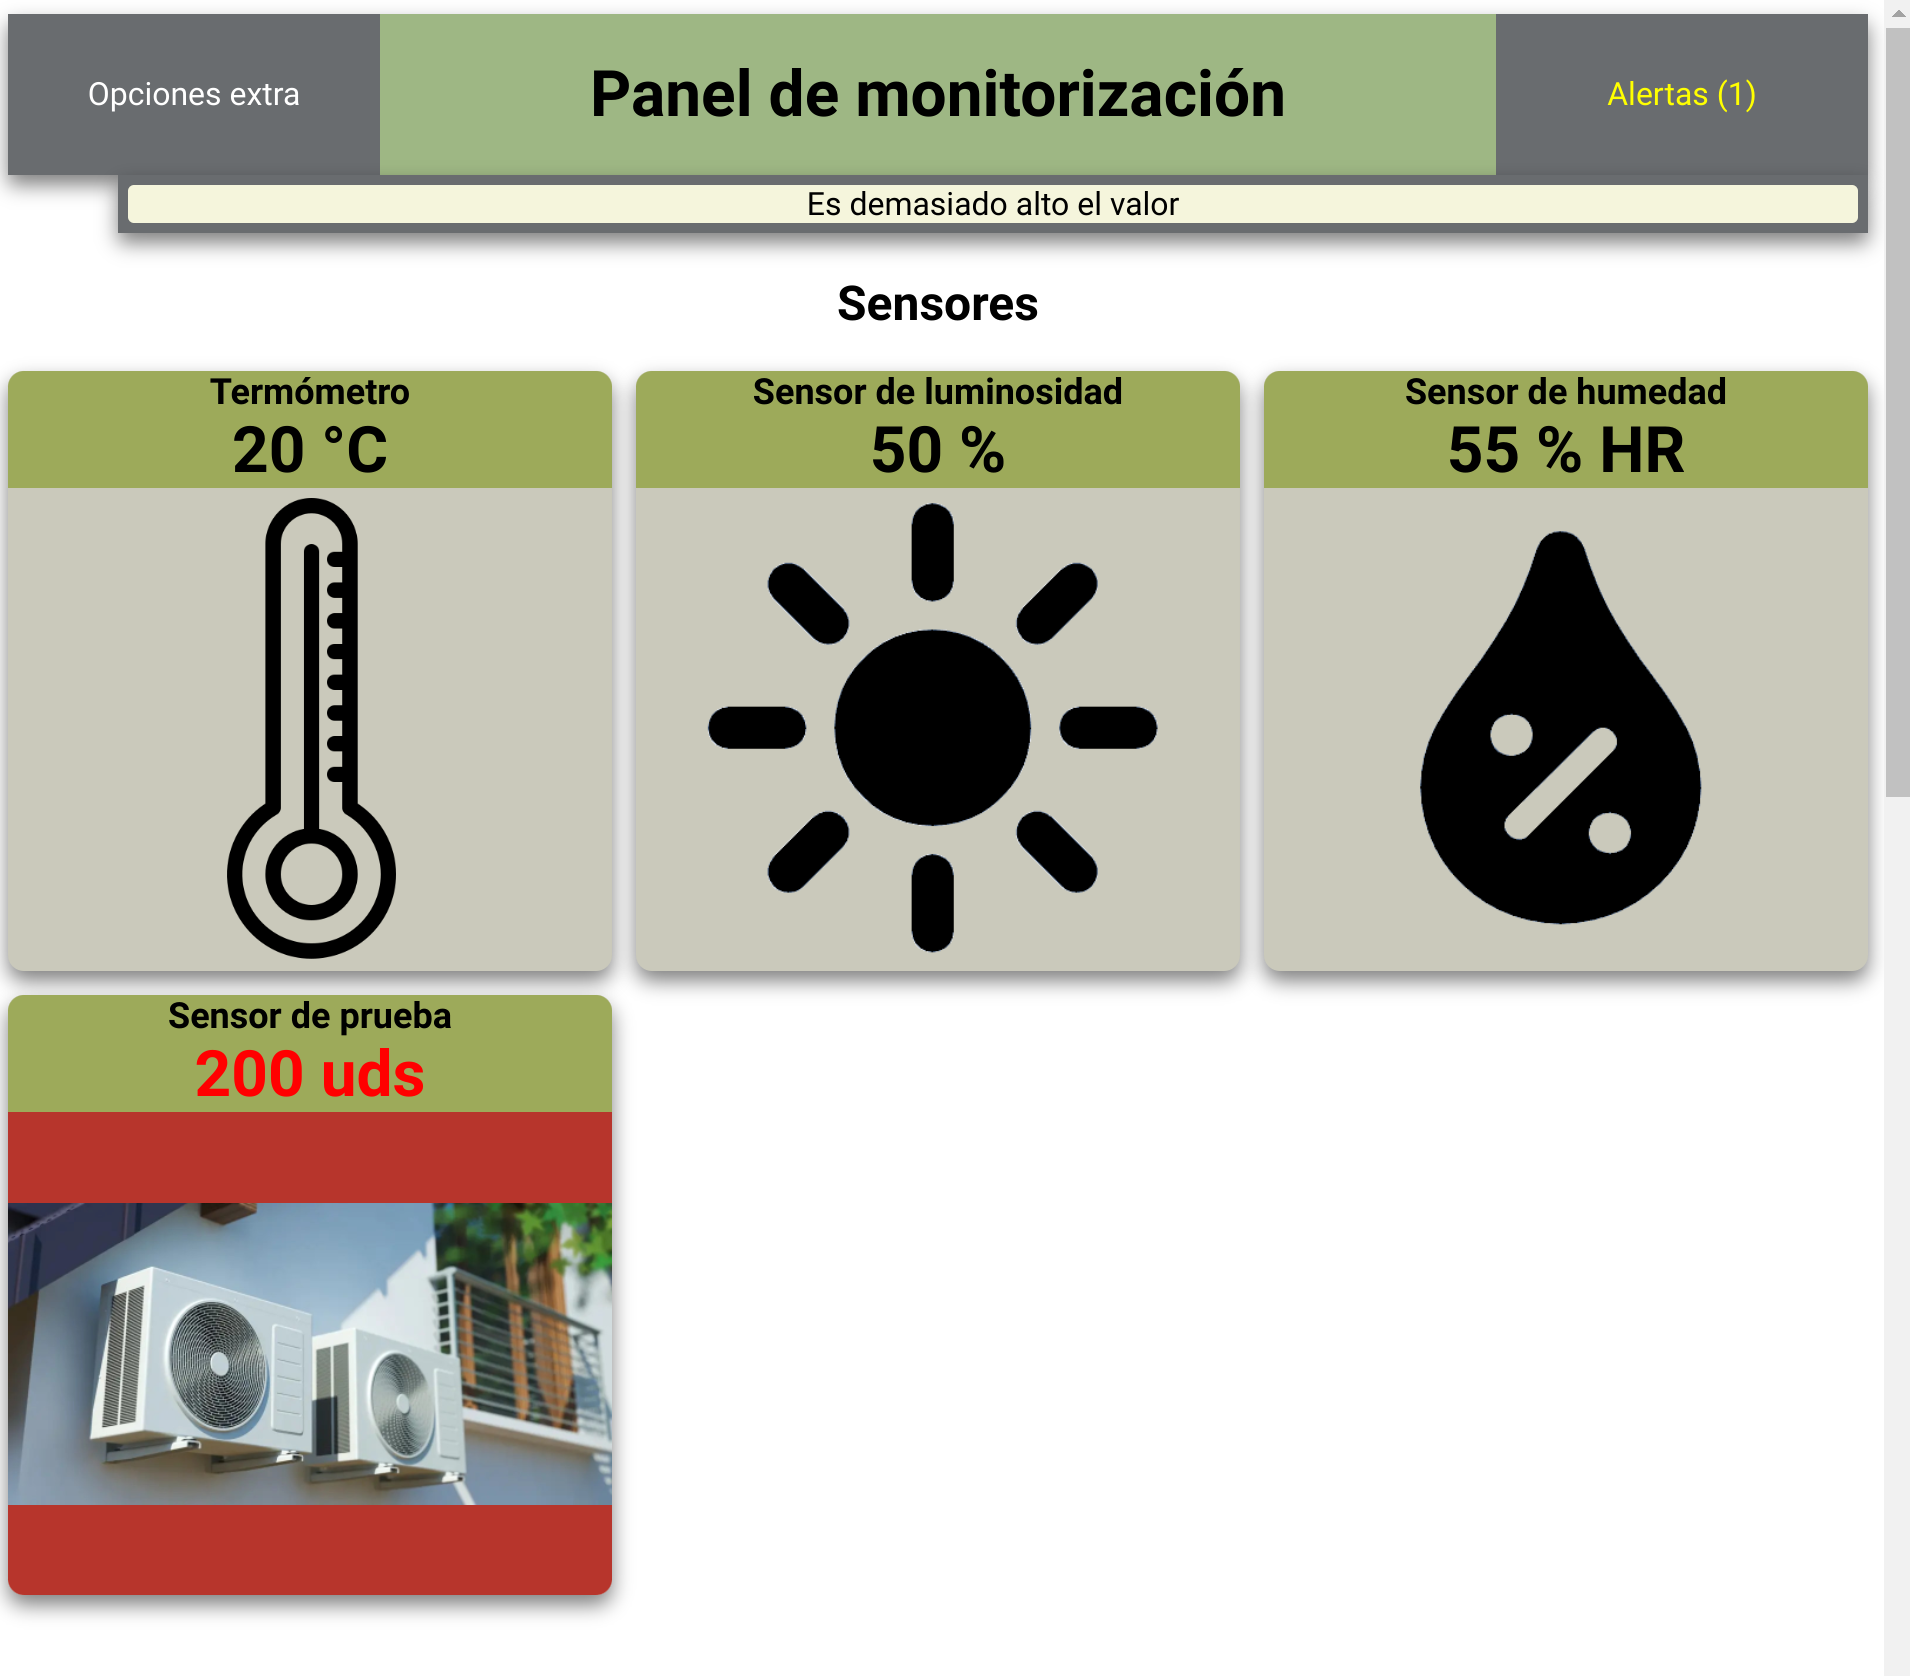
\includegraphics[width=0.7\textwidth]{images/nuevosensoralerta.png}
    \caption{Alerta producida por el nuevo sensor.}
\end{figure}

Otra cosa que he añadido ha sido una simulación básica de humedad, temperatura y luminosidad (aunque esta ultima no me convence especialmente) que se puede accionar con un boton que se encuentra en la pagina principal, debajo de los actuadores. He supuesto que es un día de verano, por lo que si todos los actuadores están apagados va a subir la temperatura y bajar la humedad. Si la ventana esta bajada supongo total oscuridad, mientras que si esta subidad, supongo un valor demasiado alto de luminosidad.

Además, cuando se acciona el aire acondicionado bjaa la temperatura, mientras que si esta el radiador sube. Si esta encendido el humidificador sube la humedad y si esta encendido el deshumidificador baja. He supuesto que si los dos aparatos de cada pareja anteriomente mencionada están encendidos, se mantienen sus valores, excepto para el caso de la ventana que si esta subida aumenta un poco la temperatura tambien.

%FOTOS DE AUTOREGULACION
\begin{figure}[H]
    \centering
    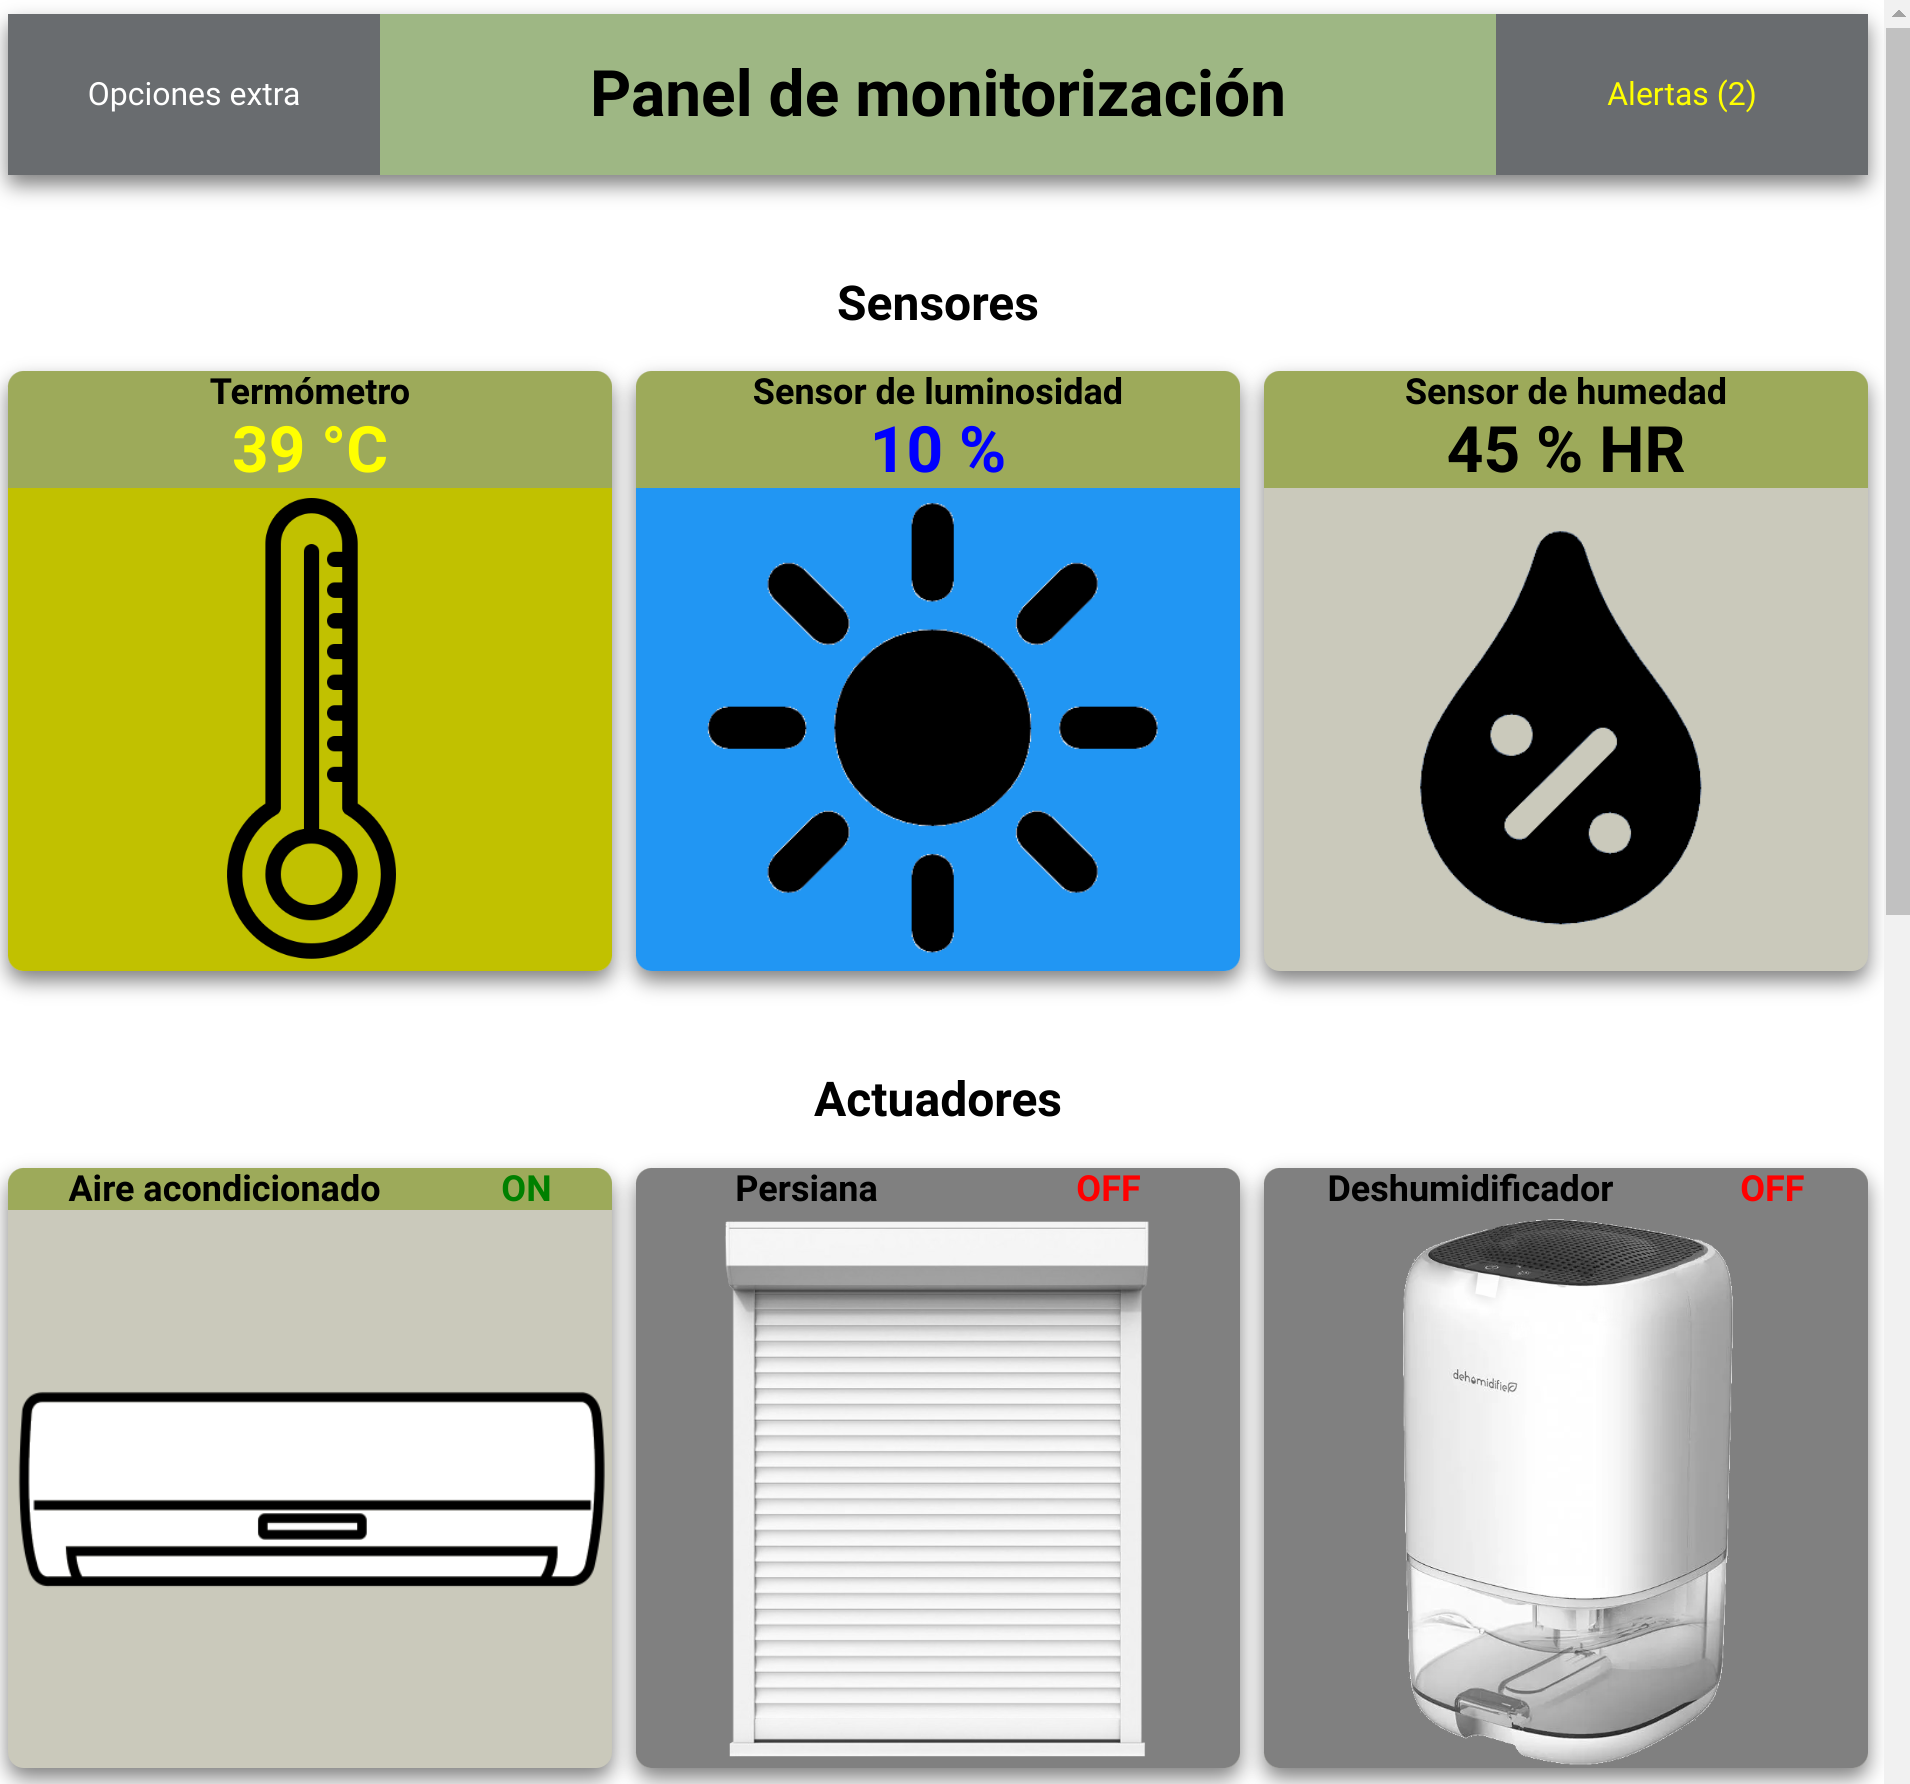
\includegraphics[width=0.7\textwidth]{images/sim.png}
    \caption{Se ha activado el aire acondicionado porque la temperatura era excesiva.}
\end{figure}

En la parte superior izquierda de la página principal hay un texto que pone ``Opciones extra'' que si se pulsa sobre el aparece un menu.

%MOSTRAR FOTO DEL MENU
\begin{figure}[H]
    \centering
    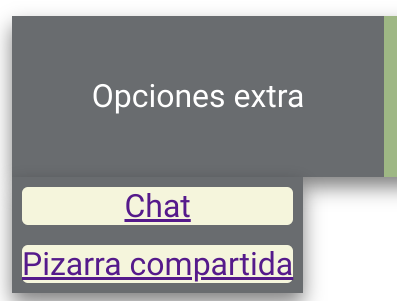
\includegraphics[width=0.4\textwidth]{images/extra.png}
    \caption{Menu con opciones extra.}
\end{figure}

La parte del chat consiste en un grupo en el que todas las personas que esten registradas se pueden mandar y recibir mensajes a la vez.

Antes que nada se presenta al usuario con una pantalla de login/registro.

En caso de tener credenciales incorrectos en el login o tener un nombre existente en el registro, se muestra un error.

\begin{figure}[H]
    \centering
    \begin{minipage}[H]{0.49\textwidth}
        \centering
        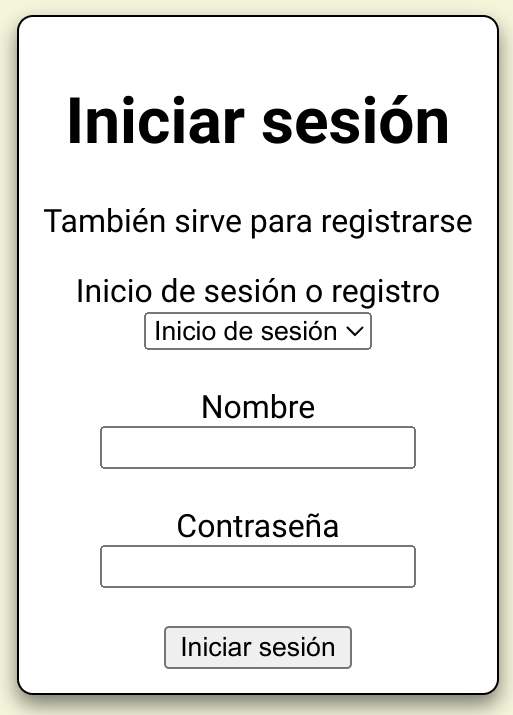
\includegraphics[width=\textwidth]{images/login.png}
        \caption{Pantalla de login.}
    \end{minipage}
    \hfill
    \begin{minipage}[H]{0.49\textwidth}
        \centering
        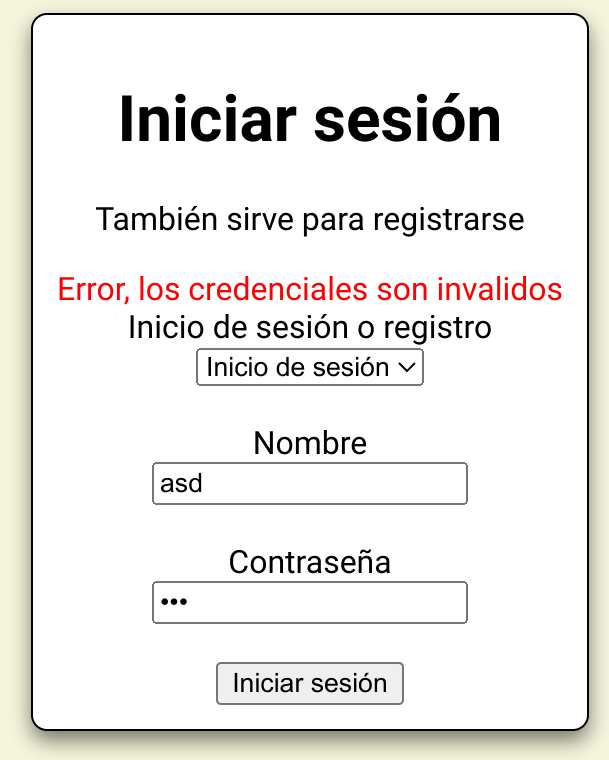
\includegraphics[width=\textwidth]{images/errorlogin.png}
        \caption{Error de credenciales de login.}
    \end{minipage}
\end{figure}

Cuando el usuario inicia sesión es presentado al chat con todos los mensajes anteriores y además es capaz de poder enviar más.

%MOSTRAR FOTO DEL CHAT
\begin{figure}[H]
    \centering
    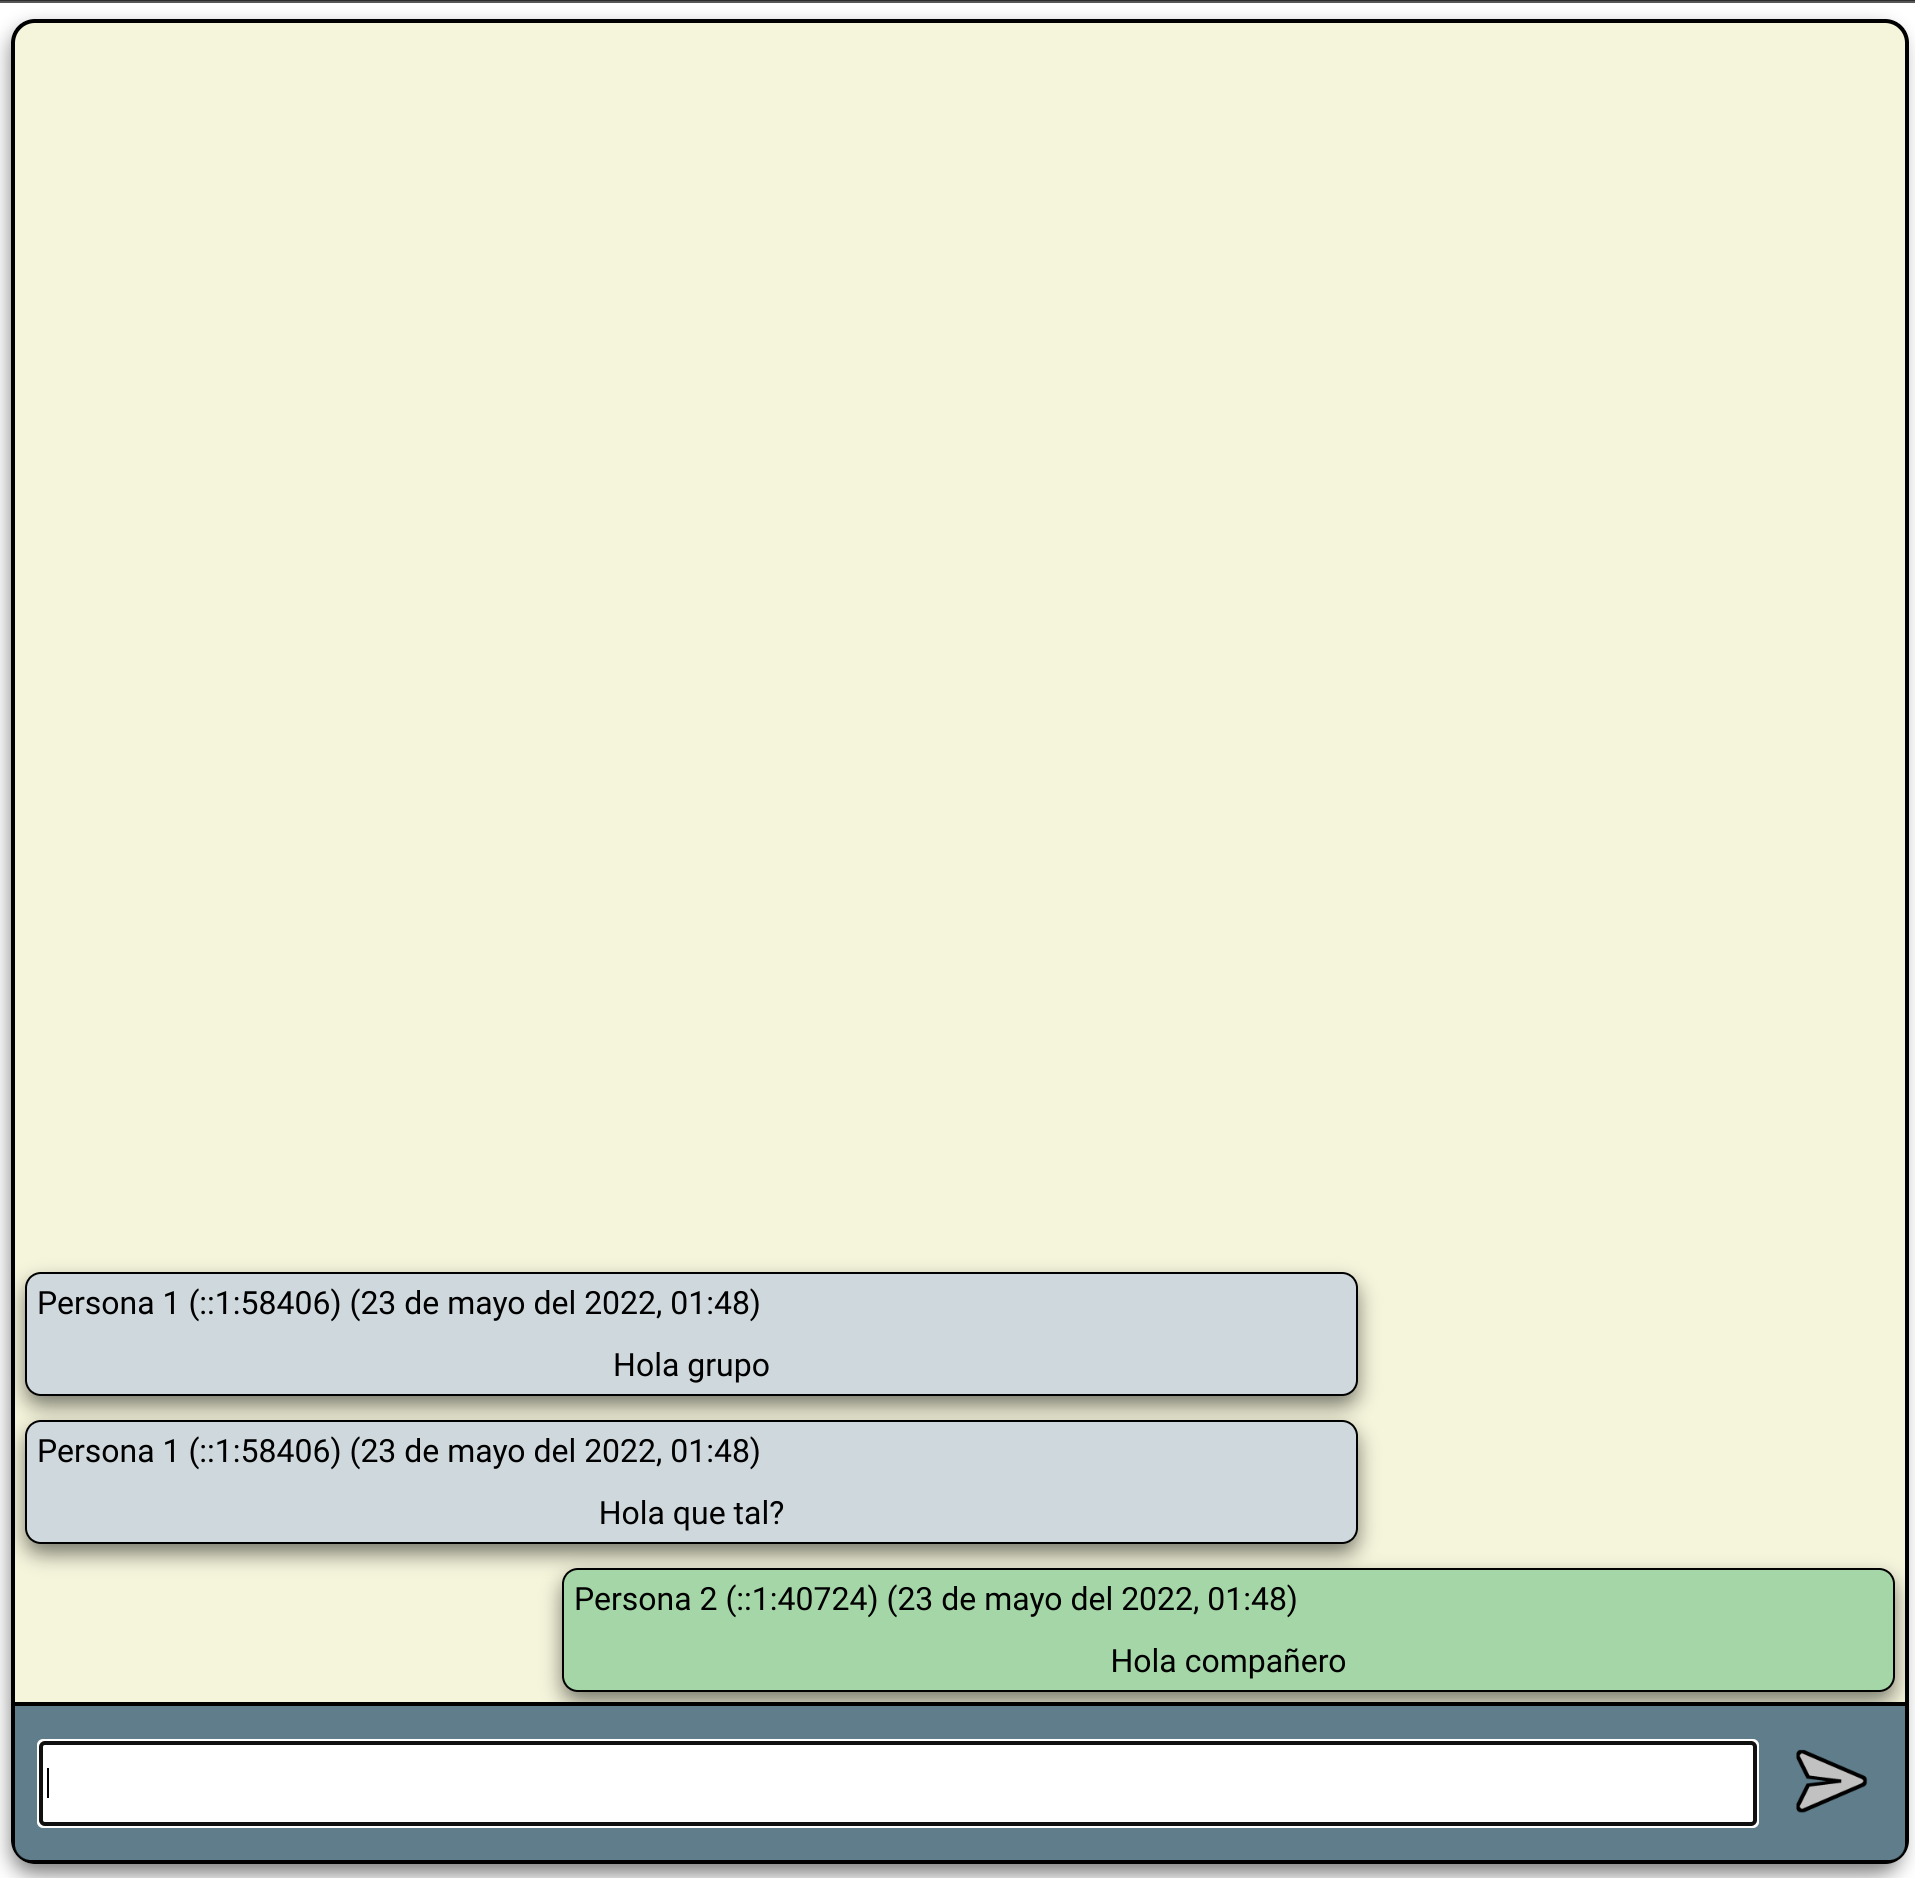
\includegraphics[width=0.7\textwidth]{images/chatmsg.png}
    \caption{Ejemplo de conversacion.}
\end{figure}

Además, si el usuario sale del chat, sin cerrar pestaña, puede seguir entrando sin iniciar sesión de nuevo. Esto se consigue utilizando ``sessionStorage'' de JavaScript.

También he puesto un censurador de palabrotas que pone con el símbolo `*' la palabra que detecte como mala.

%FOTO DEL CENSURADOR DE PALABROTAS
\begin{figure}[H]
    \centering
    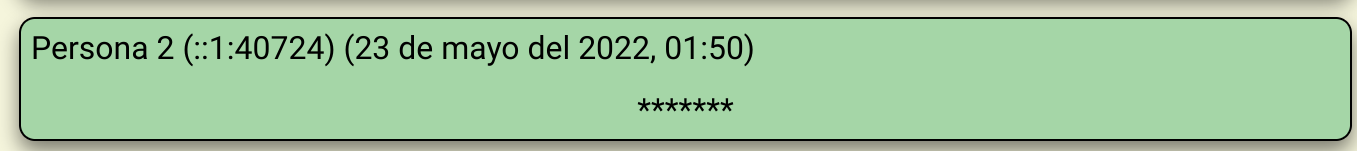
\includegraphics[width=0.7\textwidth]{images/censura.png}
    \caption{Palabrota censurada.}
\end{figure}

Para implementar esto he creado dos colecciones: una para los usuarios registrados y otra para los mensajes enviados.

Los eventos añadidos son los siguientes:

\begin{itemize}
    \item \textbf{recibir-todos-msgs: }Evento que obtiene todos los mensajes de la base de datos. Solo se acciona si el servidor ha comprobado que los credenciales son correctos.
    \item \textbf{recibir-msg: }Recibe el mensaje que ha enviado un usuario. En el servidor además se guarda en la base de datos y se comprueba que lo ha enviado una persona que existe.
    \item \textbf{comprobar-cuenta: }Comprueba que los credenciales introducidos para iniciar sesión son válidos, en caso correcto, el cliente cambia la pantalla de login a la del chat y envía una peticion a ``recibir-todos-msgs'' con sus credenciales para recibir los mensajes de chat.
    \item \textbf{crear-cuenta: }El servidor crea la cuenta almacenandola en la base de datos y devuelve true, en otro caso false. En el cliente al recibir el evento, realiza lo mismo que ``comprobar-cuenta''.
\end{itemize}    

Además, para la parte de inicio de sesión persistente, se tiene una parte ``main'' que se ejecuta si ve que tiene credenciales guardados en la sesión.

%MAS FOTOS DEL CHAT

La otra opcion de ``Opciones extra'' es la de una pizarra digital del estilo de ``Google Jamboard''. Varios usuarios pueden dibujar a la vez y cada uno ve en su pantalla los dibujos del otro en tiempo real. Además tiene 3 colores, una goma de borrar, 3 grosores y una opcion de borrar todo el lienzo. Todo esto lo ven tambien los demas.

Para la implementacion de esto, he tenido que hacer un ``canvas'' con HTML y tener en cuenta que un dibujo es un conjunto de lineas, y que una linea esta formada por dos puntos. Por tanto, hay que ser consciente de que el servidor debe almacenar un array de JSON con el grosor y el color del trazo y con el punto de comienzo y de fin de la linea.

%FOTO DE LA PIZARRA EN DOS VENTANAS DISTINTAS
\begin{figure}[H]
    \centering
    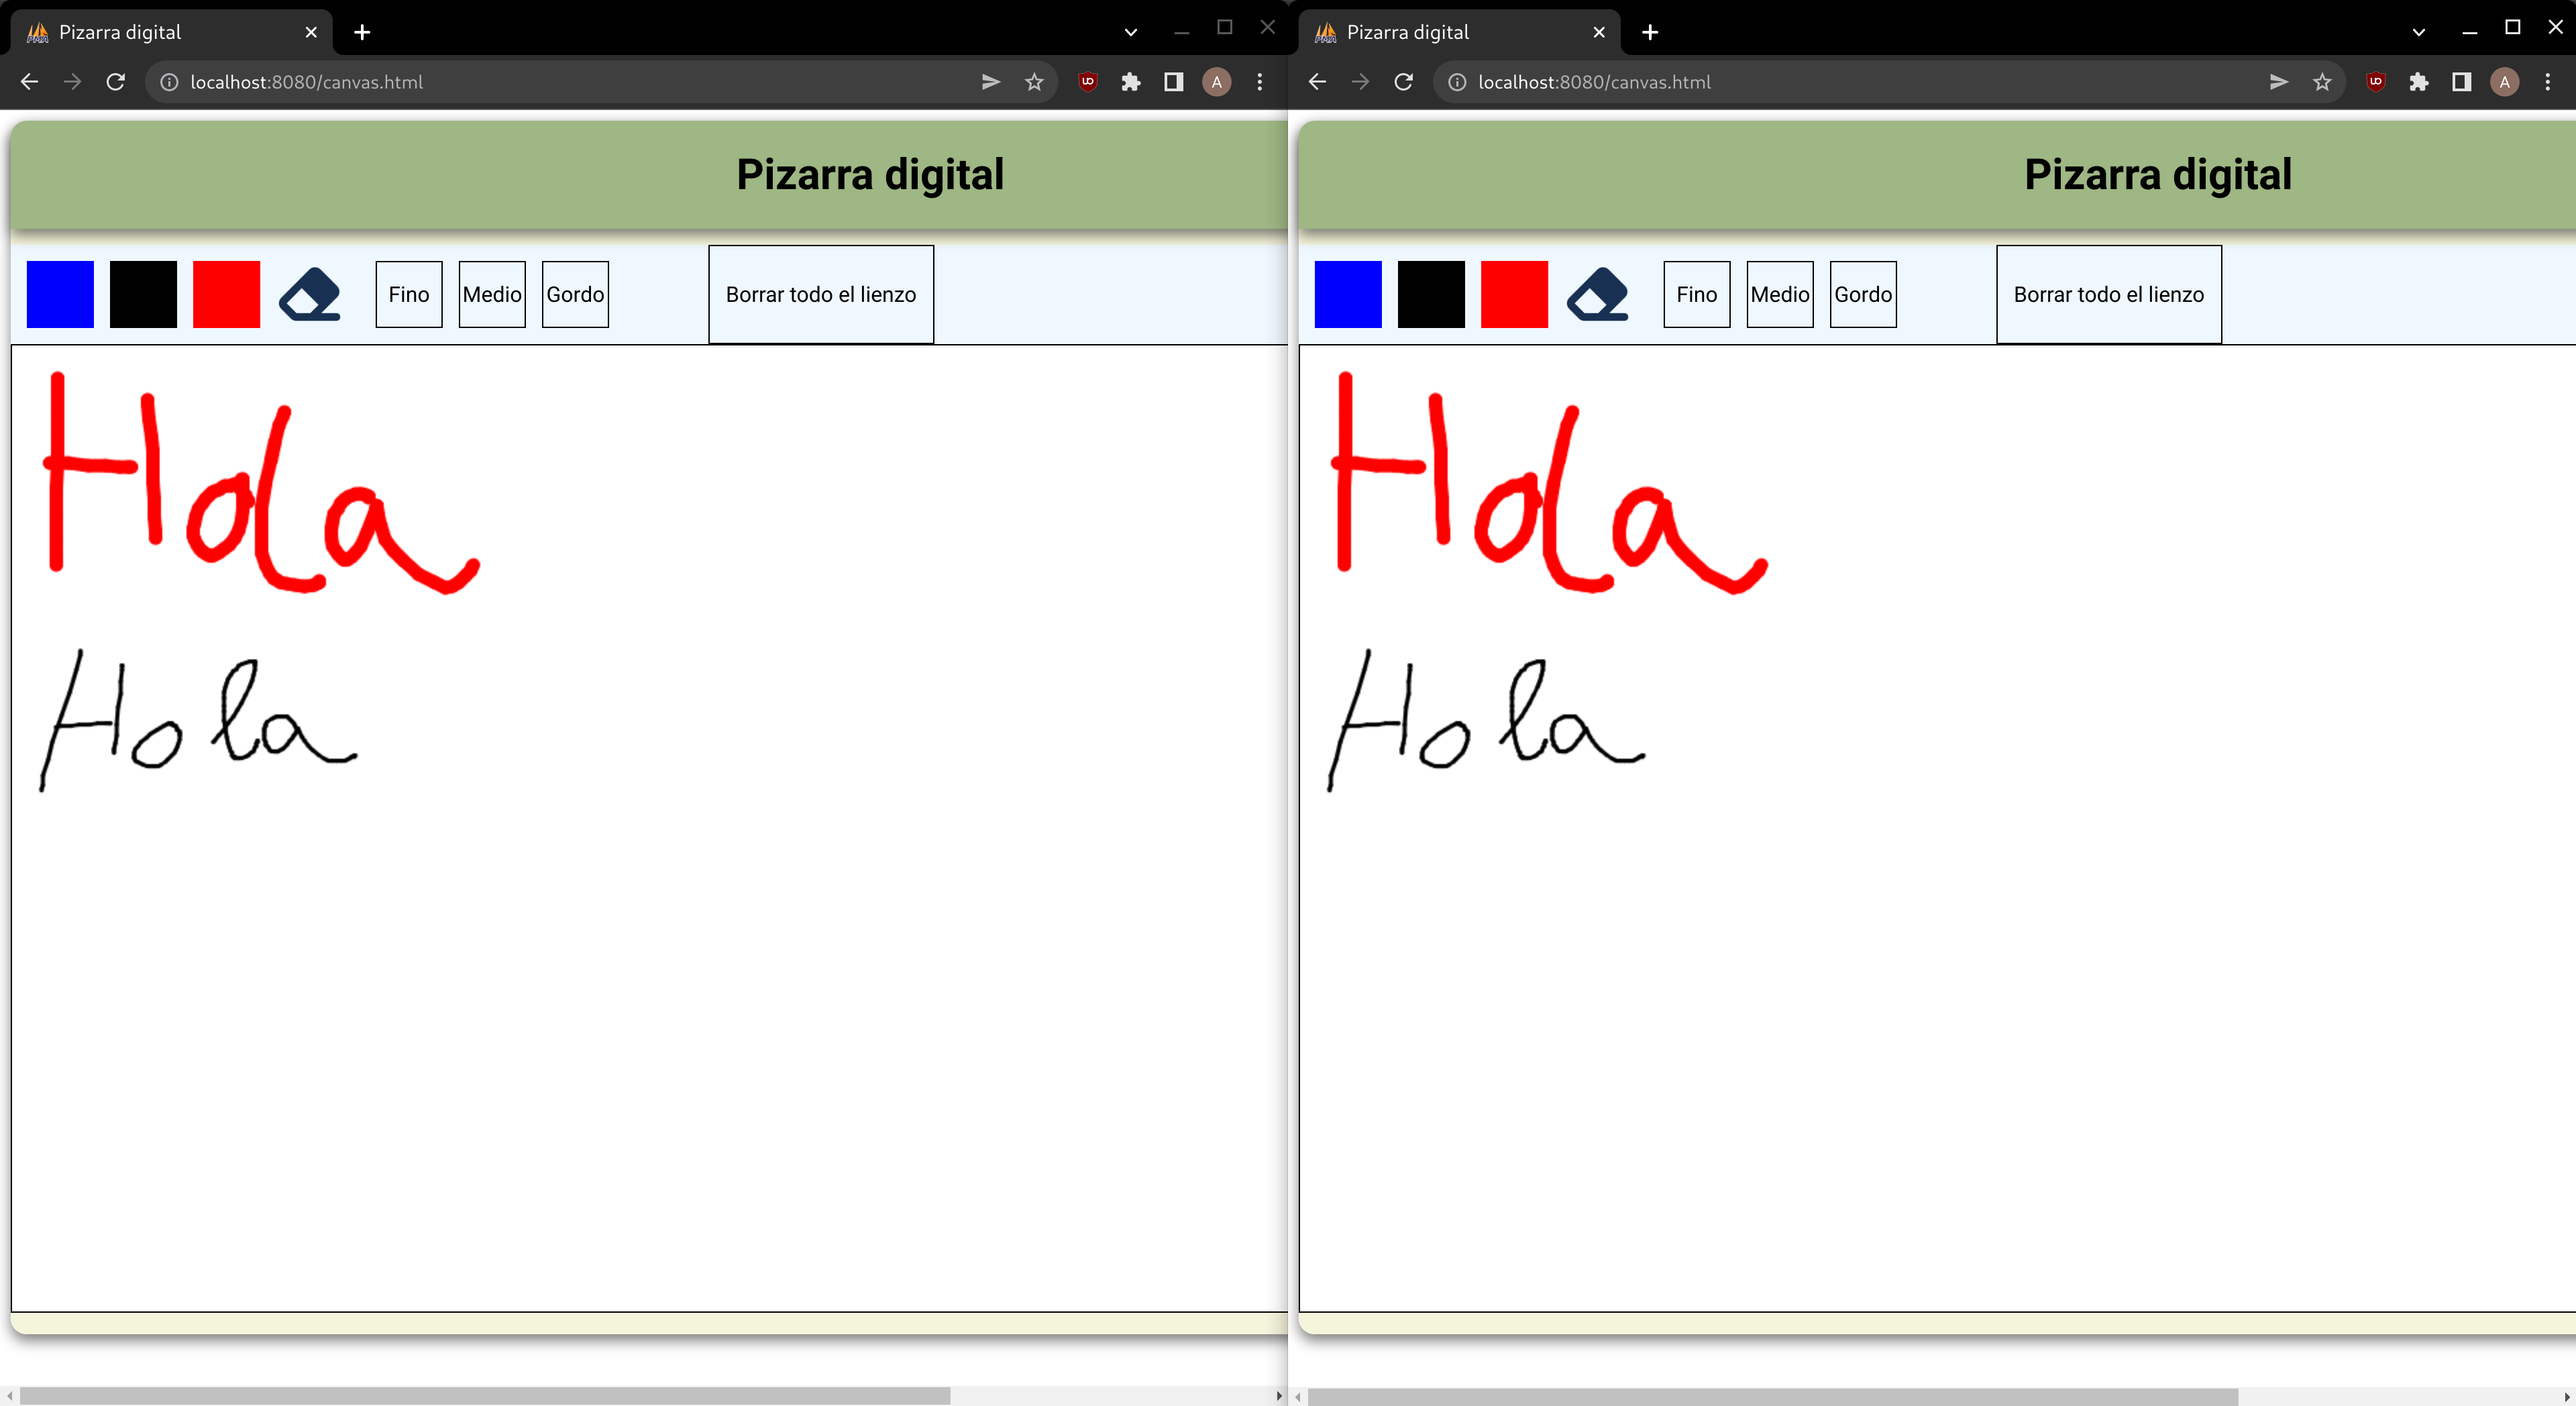
\includegraphics[width=0.7\textwidth]{images/pizarra.png}
    \caption{Pizarra de los dos clientes. Se puede ver que tienen el mismo dibujo}
\end{figure}


Para ello se han creado los siguientes eventos:

\begin{itemize}
    \item \textbf{update-pizarra: }Actualiza la pizarra con los nuevos trazos que se han introducido, ya sea por el propio usuario o por otro. Además se pinta del color que ha seleccionado el usuario que lo ha realizado.
    \item \textbf{limpiar-lienzo: }Limpia el lienzo de todos los clientes y elimina todos los datos del array del lienzo en el servidor.
\end{itemize}

Cuando un cliente nuevo se conecta, el servidor le envia todos los trazos mediante el evento ``update-pizarra''. A partir de ahi, ya el usuario puede pintar como los demas.

%OTRA FOTO MAS

Para finalizar la memoria, me gustaría mencionar que soy consciente de que el sistema no está libre de bugs, he intentado eliminar todos los que he podido. También no es lo más eficiente que me gustaría que fuera, repitiendo mucho código y seguramente con eventos que se podrían encapsular en otros.

Además, también queria hacer un bot de Twitter que escribiese tweets con todas las alertas en un momento; sin embargo pedí la cuenta de desarrollador demasiado tarde (sábado 21 de mayo) y no me ha dado tiempo a implementarlo.

\end{document}